% CS301 Week 2 -- what does an operation cost: T(n), asymptotic notation,
% and best/worst/average case.
% Difficulty: core. Page-grounded in Sedgewick2011 pp.172/187 (analysis opener +
% orders-of-growth table). Karumanchi2017 Ch.1 (pp.16-61 PDF) covers the same
% toolkit chapter-boundary-verified. Horowitz & Sahni Ch.1 and Neapolitan &
% Naimipour Ch.1-2 are chapter-level only (per textbook-grounding.md).
% Continues the expression-processor thread from Week 1: how do we predict
% whether the calculator's symbol-table lookup stays fast as the table grows?

\documentclass[aspectratio=169]{beamer}
% =============================================================================
% Preambles/header.tex — shared LaTeX/Beamer preamble for this project
%
% Use from a Beamer lecture by prepending:
%     % =============================================================================
% Preambles/header.tex — shared LaTeX/Beamer preamble for this project
%
% Use from a Beamer lecture by prepending:
%     % =============================================================================
% Preambles/header.tex — shared LaTeX/Beamer preamble for this project
%
% Use from a Beamer lecture by prepending:
%     \input{header}
% and compiling with TEXINPUTS=../Preambles:$TEXINPUTS (the /compile-latex
% skill does this automatically).
%
% PALETTE CONTRACT. Color names defined here MUST match the names in
% Quarto/theme-template.scss so Beamer and Quarto renderings use the same
% palette. The scripts/check-palette-sync.sh script enforces this.
%
% To customize: edit the HEX values below AND the matching $variable in
% Quarto/theme-template.scss, then run scripts/check-palette-sync.sh.
%
% TITLE PAGE. A formal, serif (Libertine) title-page template is defined in
% the Beamer-only block below (\setbeamertemplate{title page}) -- title,
% subtitle, a thin gold rule, then \author/\institute/\date. Frametitle and
% body text remain on Beamer's sans-serif default. No SCSS counterpart is
% needed for this (font/layout only, no new colors).
% =============================================================================

% -----------------------------------------------------------------------------
% Engine detection + encoding
%
% Our /compile-latex skill uses XeLaTeX, where inputenc is unnecessary and
% can produce encoding warnings. Only load inputenc under pdfTeX.
% -----------------------------------------------------------------------------
\usepackage{iftex}
\ifPDFTeX
  \usepackage[utf8]{inputenc}
\fi

\usepackage{amsmath, amssymb, amsthm}
\usepackage{booktabs}
\usepackage{graphicx}

% -----------------------------------------------------------------------------
% Serif face for the title page (formal/academic look). Linux Libertine is
% XeLaTeX- and pdfTeX-safe and redefines \rmdefault, so \rmfamily picks it up
% everywhere \rmfamily is used explicitly. Body text and frametitles stay on
% Beamer's own sans-serif default (unaffected) -- only the title-page
% \setbeamerfont{...} overrides below opt in to \rmfamily.
% -----------------------------------------------------------------------------
\usepackage{libertine}

% -----------------------------------------------------------------------------
% PALETTE — mirrors Quarto/theme-template.scss variable names.
% Load xcolor and define colors BEFORE anything that references them
% (notably hyperref, hypersetup, and the Beamer color assignments).
% -----------------------------------------------------------------------------
\usepackage{xcolor}

\definecolor{primary-blue}{HTML}{012169}      % headings, accents
\definecolor{primary-gold}{HTML}{B9975B}      % emphasis, borders
\definecolor{highlight-yellow}{HTML}{F2A900}  % markers, alerts
\definecolor{light-bg}{HTML}{E8EDF5}          % title / section backgrounds
\definecolor{jet}{HTML}{1A1A1A}               % body text

% Semantic colors (used in diagrams and annotations)
\definecolor{positive}{HTML}{15803D}          % good / observed / identified
\definecolor{negative}{HTML}{B91C1C}          % bad / problematic / bias
\definecolor{neutral}{HTML}{525252}           % reference / context

% Highlight accents (match .hi-* classes in the SCSS)
\definecolor{hi-slate}{HTML}{314F4F}
\definecolor{hi-green}{HTML}{2E8B57}
\definecolor{hi-red}{HTML}{C41E3A}

% Semantic aliases so skill templates and snippets can write
% \textcolor{accent}{...} without hard-coding "primary-blue".
\colorlet{accent}{primary-blue}
\colorlet{accent2}{primary-gold}

% -----------------------------------------------------------------------------
% Hyperref — loaded AFTER xcolor + palette so link colors resolve.
% -----------------------------------------------------------------------------
\usepackage{hyperref}
\hypersetup{colorlinks=true, linkcolor=primary-blue, urlcolor=primary-blue,
            citecolor=primary-blue, pdfborder={0 0 0}}

% -----------------------------------------------------------------------------
% Course code — set once per deck (after \input{header}, before \begin{document})
% via \coursecode{CS401}. Shown in the footer on every slide so a deck's course
% is identifiable without opening the title page. Empty by default.
% -----------------------------------------------------------------------------
\makeatletter
\newcommand{\coursecode}[1]{\gdef\@coursecodetext{#1}}
\gdef\@coursecodetext{}
\makeatother

% -----------------------------------------------------------------------------
% Beamer theme assignments (only apply under Beamer).
%
% We detect Beamer via \@ifclassloaded{beamer}, which is the documented,
% non-internal way. This must be wrapped in \makeatletter/\makeatother
% because \@ifclassloaded contains an @-catcode character.
% -----------------------------------------------------------------------------
\makeatletter
\@ifclassloaded{beamer}{%
  \usefonttheme{professionalfonts}
  \setbeamercolor{structure}{fg=primary-blue}
  \setbeamercolor{frametitle}{fg=primary-blue}
  \setbeamercolor{title}{fg=primary-blue}
  \setbeamercolor{subtitle}{fg=primary-gold}
  \setbeamercolor{author}{fg=primary-blue}
  \setbeamercolor{institute}{fg=neutral}
  \setbeamercolor{date}{fg=primary-gold}
  \setbeamercolor{itemize item}{fg=primary-blue}
  \setbeamercolor{itemize subitem}{fg=primary-gold}
  \setbeamercolor{alerted text}{fg=primary-gold}
  \setbeamercolor{block title}{fg=white, bg=primary-blue}
  \setbeamercolor{block body}{bg=light-bg}
  % Semantic block variants: block=definition/concept (blue), exampleblock=
  % worked example (green/positive), alertblock=key takeaway or caution (gold).
  % Keep to <=2 colored boxes per slide across ALL three variants (INV-7).
  \setbeamercolor{block title example}{fg=white, bg=positive}
  \setbeamercolor{block body example}{bg=light-bg}
  \setbeamercolor{block title alerted}{fg=white, bg=primary-gold}
  \setbeamercolor{block body alerted}{bg=light-bg}

  % ---------------------------------------------------------------------------
  % Formal title page: serif (Libertine, via \rmfamily) for title-page
  % elements only. Body text, itemize, and frametitle are intentionally left
  % on Beamer's sans-serif default -- \usebeamerfont{title} is also what
  % \transitionslide (below) uses for its big centered text, so section
  % transitions pick up the same serif treatment for free.
  % ---------------------------------------------------------------------------
  \setbeamerfont{title}{family=\rmfamily, series=\bfseries, size=\Large}
  \setbeamerfont{subtitle}{family=\rmfamily, shape=\itshape, size=\normalsize}
  \setbeamerfont{author}{family=\rmfamily, size=\normalsize}
  \setbeamerfont{institute}{family=\rmfamily, size=\scriptsize}
  \setbeamerfont{date}{family=\rmfamily, size=\scriptsize}

  \setbeamertemplate{title page}{
    \vfill
    \begin{center}
      {\usebeamerfont{title}\usebeamercolor[fg]{title}\inserttitle\par}
      \vspace{0.15cm}
      {\usebeamerfont{subtitle}\usebeamercolor[fg]{subtitle}\insertsubtitle\par}
      \vspace{0.45cm}
      {\color{primary-gold}\rule{0.42\textwidth}{0.6pt}\par}
      \vspace{0.45cm}
      {\usebeamerfont{author}\usebeamercolor[fg]{author}\insertauthor\par}
      \vspace{0.35cm}
      {\usebeamerfont{institute}\usebeamercolor[fg]{institute}\insertinstitute\par}
      \vspace{0.35cm}
      {\usebeamerfont{date}\usebeamercolor[fg]{date}\insertdate\par}
    \end{center}
    \vfill
  }

  % Minimal footer: course code (left) + page X / N (right), no navigation clutter
  \setbeamertemplate{navigation symbols}{}
  \setbeamertemplate{footline}{%
    \color{neutral}\footnotesize\hspace{0.7em}\@coursecodetext\hfill
    \insertframenumber/\inserttotalframenumber\hspace{0.7em}\vspace{0.3em}}
}{}
\makeatother

% -----------------------------------------------------------------------------
% TikZ setup — libraries the snippet gallery uses
% -----------------------------------------------------------------------------
\usepackage{tikz}
\usetikzlibrary{arrows.meta, positioning, calc, decorations.pathreplacing,
                fit, shapes.geometric, backgrounds}

% Shared TikZ styles — snippets and hand-written diagrams can pick these up
% via `\begin{tikzpicture}[every node/.style={...}]` or by naming specific
% styles (e.g., `\node[dag-node] (X) at (0,0) {X};`).
\tikzset{
  % Node styles for causal DAGs and similar
  dag-node/.style = {
    draw=primary-blue, fill=light-bg, rounded corners=2pt,
    minimum width=1.2cm, minimum height=0.9cm, align=center, font=\small
  },
  decision-node/.style = {
    draw=primary-gold, fill=white, diamond, aspect=1.8,
    minimum width=1.8cm, minimum height=1.2cm, align=center, font=\small,
    inner sep=1pt
  },
  % Edge styles — observed vs counterfactual
  observed-edge/.style = {-{Latex[length=2.5mm]}, thick, draw=jet},
  counterfactual-edge/.style = {-{Latex[length=2.5mm]}, thick, draw=neutral, dashed},
  confound-edge/.style = {-{Latex[length=2.5mm]}, thick, draw=negative, dashed},
  % Data-point styles for plots
  observed-dot/.style = {fill=primary-blue, draw=primary-blue, circle, inner sep=1.2pt},
  counterfactual-dot/.style = {fill=white, draw=neutral, circle, inner sep=1.2pt}
}

% -----------------------------------------------------------------------------
% Convenience macros
% -----------------------------------------------------------------------------
\newcommand{\muted}[1]{\textcolor{neutral}{#1}}
\newcommand{\key}[1]{\textcolor{primary-gold}{\textbf{#1}}}
\newcommand{\good}[1]{\textcolor{positive}{#1}}
\newcommand{\bad}[1]{\textcolor{negative}{#1}}

% Standout frame macro: full-bleed dark background for section transitions.
% Beamer-only (uses \begin{frame}/\setbeamercolor/\usebeamerfont) -- do not
% call from an article-class file (e.g. Notes/<CODE>/*-notes.tex). \muted,
% \key, \good, \bad, and \coursecode above are plain xcolor/gdef and are
% safe to use from either class; verified when Notes/article-class support
% was added.
% Expand: \transitionslide{Your transition title}
\newcommand{\transitionslide}[1]{%
  \begingroup
  \setbeamercolor{background canvas}{bg=primary-blue}
  \begin{frame}[plain]
    \centering
    \vfill
    {\usebeamerfont{title}\color{white}\Large #1\par}
    \vfill
  \end{frame}
  \endgroup
}

% and compiling with TEXINPUTS=../Preambles:$TEXINPUTS (the /compile-latex
% skill does this automatically).
%
% PALETTE CONTRACT. Color names defined here MUST match the names in
% Quarto/theme-template.scss so Beamer and Quarto renderings use the same
% palette. The scripts/check-palette-sync.sh script enforces this.
%
% To customize: edit the HEX values below AND the matching $variable in
% Quarto/theme-template.scss, then run scripts/check-palette-sync.sh.
%
% TITLE PAGE. A formal, serif (Libertine) title-page template is defined in
% the Beamer-only block below (\setbeamertemplate{title page}) -- title,
% subtitle, a thin gold rule, then \author/\institute/\date. Frametitle and
% body text remain on Beamer's sans-serif default. No SCSS counterpart is
% needed for this (font/layout only, no new colors).
% =============================================================================

% -----------------------------------------------------------------------------
% Engine detection + encoding
%
% Our /compile-latex skill uses XeLaTeX, where inputenc is unnecessary and
% can produce encoding warnings. Only load inputenc under pdfTeX.
% -----------------------------------------------------------------------------
\usepackage{iftex}
\ifPDFTeX
  \usepackage[utf8]{inputenc}
\fi

\usepackage{amsmath, amssymb, amsthm}
\usepackage{booktabs}
\usepackage{graphicx}

% -----------------------------------------------------------------------------
% Serif face for the title page (formal/academic look). Linux Libertine is
% XeLaTeX- and pdfTeX-safe and redefines \rmdefault, so \rmfamily picks it up
% everywhere \rmfamily is used explicitly. Body text and frametitles stay on
% Beamer's own sans-serif default (unaffected) -- only the title-page
% \setbeamerfont{...} overrides below opt in to \rmfamily.
% -----------------------------------------------------------------------------
\usepackage{libertine}

% -----------------------------------------------------------------------------
% PALETTE — mirrors Quarto/theme-template.scss variable names.
% Load xcolor and define colors BEFORE anything that references them
% (notably hyperref, hypersetup, and the Beamer color assignments).
% -----------------------------------------------------------------------------
\usepackage{xcolor}

\definecolor{primary-blue}{HTML}{012169}      % headings, accents
\definecolor{primary-gold}{HTML}{B9975B}      % emphasis, borders
\definecolor{highlight-yellow}{HTML}{F2A900}  % markers, alerts
\definecolor{light-bg}{HTML}{E8EDF5}          % title / section backgrounds
\definecolor{jet}{HTML}{1A1A1A}               % body text

% Semantic colors (used in diagrams and annotations)
\definecolor{positive}{HTML}{15803D}          % good / observed / identified
\definecolor{negative}{HTML}{B91C1C}          % bad / problematic / bias
\definecolor{neutral}{HTML}{525252}           % reference / context

% Highlight accents (match .hi-* classes in the SCSS)
\definecolor{hi-slate}{HTML}{314F4F}
\definecolor{hi-green}{HTML}{2E8B57}
\definecolor{hi-red}{HTML}{C41E3A}

% Semantic aliases so skill templates and snippets can write
% \textcolor{accent}{...} without hard-coding "primary-blue".
\colorlet{accent}{primary-blue}
\colorlet{accent2}{primary-gold}

% -----------------------------------------------------------------------------
% Hyperref — loaded AFTER xcolor + palette so link colors resolve.
% -----------------------------------------------------------------------------
\usepackage{hyperref}
\hypersetup{colorlinks=true, linkcolor=primary-blue, urlcolor=primary-blue,
            citecolor=primary-blue, pdfborder={0 0 0}}

% -----------------------------------------------------------------------------
% Course code — set once per deck (after % =============================================================================
% Preambles/header.tex — shared LaTeX/Beamer preamble for this project
%
% Use from a Beamer lecture by prepending:
%     \input{header}
% and compiling with TEXINPUTS=../Preambles:$TEXINPUTS (the /compile-latex
% skill does this automatically).
%
% PALETTE CONTRACT. Color names defined here MUST match the names in
% Quarto/theme-template.scss so Beamer and Quarto renderings use the same
% palette. The scripts/check-palette-sync.sh script enforces this.
%
% To customize: edit the HEX values below AND the matching $variable in
% Quarto/theme-template.scss, then run scripts/check-palette-sync.sh.
%
% TITLE PAGE. A formal, serif (Libertine) title-page template is defined in
% the Beamer-only block below (\setbeamertemplate{title page}) -- title,
% subtitle, a thin gold rule, then \author/\institute/\date. Frametitle and
% body text remain on Beamer's sans-serif default. No SCSS counterpart is
% needed for this (font/layout only, no new colors).
% =============================================================================

% -----------------------------------------------------------------------------
% Engine detection + encoding
%
% Our /compile-latex skill uses XeLaTeX, where inputenc is unnecessary and
% can produce encoding warnings. Only load inputenc under pdfTeX.
% -----------------------------------------------------------------------------
\usepackage{iftex}
\ifPDFTeX
  \usepackage[utf8]{inputenc}
\fi

\usepackage{amsmath, amssymb, amsthm}
\usepackage{booktabs}
\usepackage{graphicx}

% -----------------------------------------------------------------------------
% Serif face for the title page (formal/academic look). Linux Libertine is
% XeLaTeX- and pdfTeX-safe and redefines \rmdefault, so \rmfamily picks it up
% everywhere \rmfamily is used explicitly. Body text and frametitles stay on
% Beamer's own sans-serif default (unaffected) -- only the title-page
% \setbeamerfont{...} overrides below opt in to \rmfamily.
% -----------------------------------------------------------------------------
\usepackage{libertine}

% -----------------------------------------------------------------------------
% PALETTE — mirrors Quarto/theme-template.scss variable names.
% Load xcolor and define colors BEFORE anything that references them
% (notably hyperref, hypersetup, and the Beamer color assignments).
% -----------------------------------------------------------------------------
\usepackage{xcolor}

\definecolor{primary-blue}{HTML}{012169}      % headings, accents
\definecolor{primary-gold}{HTML}{B9975B}      % emphasis, borders
\definecolor{highlight-yellow}{HTML}{F2A900}  % markers, alerts
\definecolor{light-bg}{HTML}{E8EDF5}          % title / section backgrounds
\definecolor{jet}{HTML}{1A1A1A}               % body text

% Semantic colors (used in diagrams and annotations)
\definecolor{positive}{HTML}{15803D}          % good / observed / identified
\definecolor{negative}{HTML}{B91C1C}          % bad / problematic / bias
\definecolor{neutral}{HTML}{525252}           % reference / context

% Highlight accents (match .hi-* classes in the SCSS)
\definecolor{hi-slate}{HTML}{314F4F}
\definecolor{hi-green}{HTML}{2E8B57}
\definecolor{hi-red}{HTML}{C41E3A}

% Semantic aliases so skill templates and snippets can write
% \textcolor{accent}{...} without hard-coding "primary-blue".
\colorlet{accent}{primary-blue}
\colorlet{accent2}{primary-gold}

% -----------------------------------------------------------------------------
% Hyperref — loaded AFTER xcolor + palette so link colors resolve.
% -----------------------------------------------------------------------------
\usepackage{hyperref}
\hypersetup{colorlinks=true, linkcolor=primary-blue, urlcolor=primary-blue,
            citecolor=primary-blue, pdfborder={0 0 0}}

% -----------------------------------------------------------------------------
% Course code — set once per deck (after \input{header}, before \begin{document})
% via \coursecode{CS401}. Shown in the footer on every slide so a deck's course
% is identifiable without opening the title page. Empty by default.
% -----------------------------------------------------------------------------
\makeatletter
\newcommand{\coursecode}[1]{\gdef\@coursecodetext{#1}}
\gdef\@coursecodetext{}
\makeatother

% -----------------------------------------------------------------------------
% Beamer theme assignments (only apply under Beamer).
%
% We detect Beamer via \@ifclassloaded{beamer}, which is the documented,
% non-internal way. This must be wrapped in \makeatletter/\makeatother
% because \@ifclassloaded contains an @-catcode character.
% -----------------------------------------------------------------------------
\makeatletter
\@ifclassloaded{beamer}{%
  \usefonttheme{professionalfonts}
  \setbeamercolor{structure}{fg=primary-blue}
  \setbeamercolor{frametitle}{fg=primary-blue}
  \setbeamercolor{title}{fg=primary-blue}
  \setbeamercolor{subtitle}{fg=primary-gold}
  \setbeamercolor{author}{fg=primary-blue}
  \setbeamercolor{institute}{fg=neutral}
  \setbeamercolor{date}{fg=primary-gold}
  \setbeamercolor{itemize item}{fg=primary-blue}
  \setbeamercolor{itemize subitem}{fg=primary-gold}
  \setbeamercolor{alerted text}{fg=primary-gold}
  \setbeamercolor{block title}{fg=white, bg=primary-blue}
  \setbeamercolor{block body}{bg=light-bg}
  % Semantic block variants: block=definition/concept (blue), exampleblock=
  % worked example (green/positive), alertblock=key takeaway or caution (gold).
  % Keep to <=2 colored boxes per slide across ALL three variants (INV-7).
  \setbeamercolor{block title example}{fg=white, bg=positive}
  \setbeamercolor{block body example}{bg=light-bg}
  \setbeamercolor{block title alerted}{fg=white, bg=primary-gold}
  \setbeamercolor{block body alerted}{bg=light-bg}

  % ---------------------------------------------------------------------------
  % Formal title page: serif (Libertine, via \rmfamily) for title-page
  % elements only. Body text, itemize, and frametitle are intentionally left
  % on Beamer's sans-serif default -- \usebeamerfont{title} is also what
  % \transitionslide (below) uses for its big centered text, so section
  % transitions pick up the same serif treatment for free.
  % ---------------------------------------------------------------------------
  \setbeamerfont{title}{family=\rmfamily, series=\bfseries, size=\Large}
  \setbeamerfont{subtitle}{family=\rmfamily, shape=\itshape, size=\normalsize}
  \setbeamerfont{author}{family=\rmfamily, size=\normalsize}
  \setbeamerfont{institute}{family=\rmfamily, size=\scriptsize}
  \setbeamerfont{date}{family=\rmfamily, size=\scriptsize}

  \setbeamertemplate{title page}{
    \vfill
    \begin{center}
      {\usebeamerfont{title}\usebeamercolor[fg]{title}\inserttitle\par}
      \vspace{0.15cm}
      {\usebeamerfont{subtitle}\usebeamercolor[fg]{subtitle}\insertsubtitle\par}
      \vspace{0.45cm}
      {\color{primary-gold}\rule{0.42\textwidth}{0.6pt}\par}
      \vspace{0.45cm}
      {\usebeamerfont{author}\usebeamercolor[fg]{author}\insertauthor\par}
      \vspace{0.35cm}
      {\usebeamerfont{institute}\usebeamercolor[fg]{institute}\insertinstitute\par}
      \vspace{0.35cm}
      {\usebeamerfont{date}\usebeamercolor[fg]{date}\insertdate\par}
    \end{center}
    \vfill
  }

  % Minimal footer: course code (left) + page X / N (right), no navigation clutter
  \setbeamertemplate{navigation symbols}{}
  \setbeamertemplate{footline}{%
    \color{neutral}\footnotesize\hspace{0.7em}\@coursecodetext\hfill
    \insertframenumber/\inserttotalframenumber\hspace{0.7em}\vspace{0.3em}}
}{}
\makeatother

% -----------------------------------------------------------------------------
% TikZ setup — libraries the snippet gallery uses
% -----------------------------------------------------------------------------
\usepackage{tikz}
\usetikzlibrary{arrows.meta, positioning, calc, decorations.pathreplacing,
                fit, shapes.geometric, backgrounds}

% Shared TikZ styles — snippets and hand-written diagrams can pick these up
% via `\begin{tikzpicture}[every node/.style={...}]` or by naming specific
% styles (e.g., `\node[dag-node] (X) at (0,0) {X};`).
\tikzset{
  % Node styles for causal DAGs and similar
  dag-node/.style = {
    draw=primary-blue, fill=light-bg, rounded corners=2pt,
    minimum width=1.2cm, minimum height=0.9cm, align=center, font=\small
  },
  decision-node/.style = {
    draw=primary-gold, fill=white, diamond, aspect=1.8,
    minimum width=1.8cm, minimum height=1.2cm, align=center, font=\small,
    inner sep=1pt
  },
  % Edge styles — observed vs counterfactual
  observed-edge/.style = {-{Latex[length=2.5mm]}, thick, draw=jet},
  counterfactual-edge/.style = {-{Latex[length=2.5mm]}, thick, draw=neutral, dashed},
  confound-edge/.style = {-{Latex[length=2.5mm]}, thick, draw=negative, dashed},
  % Data-point styles for plots
  observed-dot/.style = {fill=primary-blue, draw=primary-blue, circle, inner sep=1.2pt},
  counterfactual-dot/.style = {fill=white, draw=neutral, circle, inner sep=1.2pt}
}

% -----------------------------------------------------------------------------
% Convenience macros
% -----------------------------------------------------------------------------
\newcommand{\muted}[1]{\textcolor{neutral}{#1}}
\newcommand{\key}[1]{\textcolor{primary-gold}{\textbf{#1}}}
\newcommand{\good}[1]{\textcolor{positive}{#1}}
\newcommand{\bad}[1]{\textcolor{negative}{#1}}

% Standout frame macro: full-bleed dark background for section transitions.
% Beamer-only (uses \begin{frame}/\setbeamercolor/\usebeamerfont) -- do not
% call from an article-class file (e.g. Notes/<CODE>/*-notes.tex). \muted,
% \key, \good, \bad, and \coursecode above are plain xcolor/gdef and are
% safe to use from either class; verified when Notes/article-class support
% was added.
% Expand: \transitionslide{Your transition title}
\newcommand{\transitionslide}[1]{%
  \begingroup
  \setbeamercolor{background canvas}{bg=primary-blue}
  \begin{frame}[plain]
    \centering
    \vfill
    {\usebeamerfont{title}\color{white}\Large #1\par}
    \vfill
  \end{frame}
  \endgroup
}
, before \begin{document})
% via \coursecode{CS401}. Shown in the footer on every slide so a deck's course
% is identifiable without opening the title page. Empty by default.
% -----------------------------------------------------------------------------
\makeatletter
\newcommand{\coursecode}[1]{\gdef\@coursecodetext{#1}}
\gdef\@coursecodetext{}
\makeatother

% -----------------------------------------------------------------------------
% Beamer theme assignments (only apply under Beamer).
%
% We detect Beamer via \@ifclassloaded{beamer}, which is the documented,
% non-internal way. This must be wrapped in \makeatletter/\makeatother
% because \@ifclassloaded contains an @-catcode character.
% -----------------------------------------------------------------------------
\makeatletter
\@ifclassloaded{beamer}{%
  \usefonttheme{professionalfonts}
  \setbeamercolor{structure}{fg=primary-blue}
  \setbeamercolor{frametitle}{fg=primary-blue}
  \setbeamercolor{title}{fg=primary-blue}
  \setbeamercolor{subtitle}{fg=primary-gold}
  \setbeamercolor{author}{fg=primary-blue}
  \setbeamercolor{institute}{fg=neutral}
  \setbeamercolor{date}{fg=primary-gold}
  \setbeamercolor{itemize item}{fg=primary-blue}
  \setbeamercolor{itemize subitem}{fg=primary-gold}
  \setbeamercolor{alerted text}{fg=primary-gold}
  \setbeamercolor{block title}{fg=white, bg=primary-blue}
  \setbeamercolor{block body}{bg=light-bg}
  % Semantic block variants: block=definition/concept (blue), exampleblock=
  % worked example (green/positive), alertblock=key takeaway or caution (gold).
  % Keep to <=2 colored boxes per slide across ALL three variants (INV-7).
  \setbeamercolor{block title example}{fg=white, bg=positive}
  \setbeamercolor{block body example}{bg=light-bg}
  \setbeamercolor{block title alerted}{fg=white, bg=primary-gold}
  \setbeamercolor{block body alerted}{bg=light-bg}

  % ---------------------------------------------------------------------------
  % Formal title page: serif (Libertine, via \rmfamily) for title-page
  % elements only. Body text, itemize, and frametitle are intentionally left
  % on Beamer's sans-serif default -- \usebeamerfont{title} is also what
  % \transitionslide (below) uses for its big centered text, so section
  % transitions pick up the same serif treatment for free.
  % ---------------------------------------------------------------------------
  \setbeamerfont{title}{family=\rmfamily, series=\bfseries, size=\Large}
  \setbeamerfont{subtitle}{family=\rmfamily, shape=\itshape, size=\normalsize}
  \setbeamerfont{author}{family=\rmfamily, size=\normalsize}
  \setbeamerfont{institute}{family=\rmfamily, size=\scriptsize}
  \setbeamerfont{date}{family=\rmfamily, size=\scriptsize}

  \setbeamertemplate{title page}{
    \vfill
    \begin{center}
      {\usebeamerfont{title}\usebeamercolor[fg]{title}\inserttitle\par}
      \vspace{0.15cm}
      {\usebeamerfont{subtitle}\usebeamercolor[fg]{subtitle}\insertsubtitle\par}
      \vspace{0.45cm}
      {\color{primary-gold}\rule{0.42\textwidth}{0.6pt}\par}
      \vspace{0.45cm}
      {\usebeamerfont{author}\usebeamercolor[fg]{author}\insertauthor\par}
      \vspace{0.35cm}
      {\usebeamerfont{institute}\usebeamercolor[fg]{institute}\insertinstitute\par}
      \vspace{0.35cm}
      {\usebeamerfont{date}\usebeamercolor[fg]{date}\insertdate\par}
    \end{center}
    \vfill
  }

  % Minimal footer: course code (left) + page X / N (right), no navigation clutter
  \setbeamertemplate{navigation symbols}{}
  \setbeamertemplate{footline}{%
    \color{neutral}\footnotesize\hspace{0.7em}\@coursecodetext\hfill
    \insertframenumber/\inserttotalframenumber\hspace{0.7em}\vspace{0.3em}}
}{}
\makeatother

% -----------------------------------------------------------------------------
% TikZ setup — libraries the snippet gallery uses
% -----------------------------------------------------------------------------
\usepackage{tikz}
\usetikzlibrary{arrows.meta, positioning, calc, decorations.pathreplacing,
                fit, shapes.geometric, backgrounds}

% Shared TikZ styles — snippets and hand-written diagrams can pick these up
% via `\begin{tikzpicture}[every node/.style={...}]` or by naming specific
% styles (e.g., `\node[dag-node] (X) at (0,0) {X};`).
\tikzset{
  % Node styles for causal DAGs and similar
  dag-node/.style = {
    draw=primary-blue, fill=light-bg, rounded corners=2pt,
    minimum width=1.2cm, minimum height=0.9cm, align=center, font=\small
  },
  decision-node/.style = {
    draw=primary-gold, fill=white, diamond, aspect=1.8,
    minimum width=1.8cm, minimum height=1.2cm, align=center, font=\small,
    inner sep=1pt
  },
  % Edge styles — observed vs counterfactual
  observed-edge/.style = {-{Latex[length=2.5mm]}, thick, draw=jet},
  counterfactual-edge/.style = {-{Latex[length=2.5mm]}, thick, draw=neutral, dashed},
  confound-edge/.style = {-{Latex[length=2.5mm]}, thick, draw=negative, dashed},
  % Data-point styles for plots
  observed-dot/.style = {fill=primary-blue, draw=primary-blue, circle, inner sep=1.2pt},
  counterfactual-dot/.style = {fill=white, draw=neutral, circle, inner sep=1.2pt}
}

% -----------------------------------------------------------------------------
% Convenience macros
% -----------------------------------------------------------------------------
\newcommand{\muted}[1]{\textcolor{neutral}{#1}}
\newcommand{\key}[1]{\textcolor{primary-gold}{\textbf{#1}}}
\newcommand{\good}[1]{\textcolor{positive}{#1}}
\newcommand{\bad}[1]{\textcolor{negative}{#1}}

% Standout frame macro: full-bleed dark background for section transitions.
% Beamer-only (uses \begin{frame}/\setbeamercolor/\usebeamerfont) -- do not
% call from an article-class file (e.g. Notes/<CODE>/*-notes.tex). \muted,
% \key, \good, \bad, and \coursecode above are plain xcolor/gdef and are
% safe to use from either class; verified when Notes/article-class support
% was added.
% Expand: \transitionslide{Your transition title}
\newcommand{\transitionslide}[1]{%
  \begingroup
  \setbeamercolor{background canvas}{bg=primary-blue}
  \begin{frame}[plain]
    \centering
    \vfill
    {\usebeamerfont{title}\color{white}\Large #1\par}
    \vfill
  \end{frame}
  \endgroup
}

% and compiling with TEXINPUTS=../Preambles:$TEXINPUTS (the /compile-latex
% skill does this automatically).
%
% PALETTE CONTRACT. Color names defined here MUST match the names in
% Quarto/theme-template.scss so Beamer and Quarto renderings use the same
% palette. The scripts/check-palette-sync.sh script enforces this.
%
% To customize: edit the HEX values below AND the matching $variable in
% Quarto/theme-template.scss, then run scripts/check-palette-sync.sh.
%
% TITLE PAGE. A formal, serif (Libertine) title-page template is defined in
% the Beamer-only block below (\setbeamertemplate{title page}) -- title,
% subtitle, a thin gold rule, then \author/\institute/\date. Frametitle and
% body text remain on Beamer's sans-serif default. No SCSS counterpart is
% needed for this (font/layout only, no new colors).
% =============================================================================

% -----------------------------------------------------------------------------
% Engine detection + encoding
%
% Our /compile-latex skill uses XeLaTeX, where inputenc is unnecessary and
% can produce encoding warnings. Only load inputenc under pdfTeX.
% -----------------------------------------------------------------------------
\usepackage{iftex}
\ifPDFTeX
  \usepackage[utf8]{inputenc}
\fi

\usepackage{amsmath, amssymb, amsthm}
\usepackage{booktabs}
\usepackage{graphicx}

% -----------------------------------------------------------------------------
% Serif face for the title page (formal/academic look). Linux Libertine is
% XeLaTeX- and pdfTeX-safe and redefines \rmdefault, so \rmfamily picks it up
% everywhere \rmfamily is used explicitly. Body text and frametitles stay on
% Beamer's own sans-serif default (unaffected) -- only the title-page
% \setbeamerfont{...} overrides below opt in to \rmfamily.
% -----------------------------------------------------------------------------
\usepackage{libertine}

% -----------------------------------------------------------------------------
% PALETTE — mirrors Quarto/theme-template.scss variable names.
% Load xcolor and define colors BEFORE anything that references them
% (notably hyperref, hypersetup, and the Beamer color assignments).
% -----------------------------------------------------------------------------
\usepackage{xcolor}

\definecolor{primary-blue}{HTML}{012169}      % headings, accents
\definecolor{primary-gold}{HTML}{B9975B}      % emphasis, borders
\definecolor{highlight-yellow}{HTML}{F2A900}  % markers, alerts
\definecolor{light-bg}{HTML}{E8EDF5}          % title / section backgrounds
\definecolor{jet}{HTML}{1A1A1A}               % body text

% Semantic colors (used in diagrams and annotations)
\definecolor{positive}{HTML}{15803D}          % good / observed / identified
\definecolor{negative}{HTML}{B91C1C}          % bad / problematic / bias
\definecolor{neutral}{HTML}{525252}           % reference / context

% Highlight accents (match .hi-* classes in the SCSS)
\definecolor{hi-slate}{HTML}{314F4F}
\definecolor{hi-green}{HTML}{2E8B57}
\definecolor{hi-red}{HTML}{C41E3A}

% Semantic aliases so skill templates and snippets can write
% \textcolor{accent}{...} without hard-coding "primary-blue".
\colorlet{accent}{primary-blue}
\colorlet{accent2}{primary-gold}

% -----------------------------------------------------------------------------
% Hyperref — loaded AFTER xcolor + palette so link colors resolve.
% -----------------------------------------------------------------------------
\usepackage{hyperref}
\hypersetup{colorlinks=true, linkcolor=primary-blue, urlcolor=primary-blue,
            citecolor=primary-blue, pdfborder={0 0 0}}

% -----------------------------------------------------------------------------
% Course code — set once per deck (after % =============================================================================
% Preambles/header.tex — shared LaTeX/Beamer preamble for this project
%
% Use from a Beamer lecture by prepending:
%     % =============================================================================
% Preambles/header.tex — shared LaTeX/Beamer preamble for this project
%
% Use from a Beamer lecture by prepending:
%     \input{header}
% and compiling with TEXINPUTS=../Preambles:$TEXINPUTS (the /compile-latex
% skill does this automatically).
%
% PALETTE CONTRACT. Color names defined here MUST match the names in
% Quarto/theme-template.scss so Beamer and Quarto renderings use the same
% palette. The scripts/check-palette-sync.sh script enforces this.
%
% To customize: edit the HEX values below AND the matching $variable in
% Quarto/theme-template.scss, then run scripts/check-palette-sync.sh.
%
% TITLE PAGE. A formal, serif (Libertine) title-page template is defined in
% the Beamer-only block below (\setbeamertemplate{title page}) -- title,
% subtitle, a thin gold rule, then \author/\institute/\date. Frametitle and
% body text remain on Beamer's sans-serif default. No SCSS counterpart is
% needed for this (font/layout only, no new colors).
% =============================================================================

% -----------------------------------------------------------------------------
% Engine detection + encoding
%
% Our /compile-latex skill uses XeLaTeX, where inputenc is unnecessary and
% can produce encoding warnings. Only load inputenc under pdfTeX.
% -----------------------------------------------------------------------------
\usepackage{iftex}
\ifPDFTeX
  \usepackage[utf8]{inputenc}
\fi

\usepackage{amsmath, amssymb, amsthm}
\usepackage{booktabs}
\usepackage{graphicx}

% -----------------------------------------------------------------------------
% Serif face for the title page (formal/academic look). Linux Libertine is
% XeLaTeX- and pdfTeX-safe and redefines \rmdefault, so \rmfamily picks it up
% everywhere \rmfamily is used explicitly. Body text and frametitles stay on
% Beamer's own sans-serif default (unaffected) -- only the title-page
% \setbeamerfont{...} overrides below opt in to \rmfamily.
% -----------------------------------------------------------------------------
\usepackage{libertine}

% -----------------------------------------------------------------------------
% PALETTE — mirrors Quarto/theme-template.scss variable names.
% Load xcolor and define colors BEFORE anything that references them
% (notably hyperref, hypersetup, and the Beamer color assignments).
% -----------------------------------------------------------------------------
\usepackage{xcolor}

\definecolor{primary-blue}{HTML}{012169}      % headings, accents
\definecolor{primary-gold}{HTML}{B9975B}      % emphasis, borders
\definecolor{highlight-yellow}{HTML}{F2A900}  % markers, alerts
\definecolor{light-bg}{HTML}{E8EDF5}          % title / section backgrounds
\definecolor{jet}{HTML}{1A1A1A}               % body text

% Semantic colors (used in diagrams and annotations)
\definecolor{positive}{HTML}{15803D}          % good / observed / identified
\definecolor{negative}{HTML}{B91C1C}          % bad / problematic / bias
\definecolor{neutral}{HTML}{525252}           % reference / context

% Highlight accents (match .hi-* classes in the SCSS)
\definecolor{hi-slate}{HTML}{314F4F}
\definecolor{hi-green}{HTML}{2E8B57}
\definecolor{hi-red}{HTML}{C41E3A}

% Semantic aliases so skill templates and snippets can write
% \textcolor{accent}{...} without hard-coding "primary-blue".
\colorlet{accent}{primary-blue}
\colorlet{accent2}{primary-gold}

% -----------------------------------------------------------------------------
% Hyperref — loaded AFTER xcolor + palette so link colors resolve.
% -----------------------------------------------------------------------------
\usepackage{hyperref}
\hypersetup{colorlinks=true, linkcolor=primary-blue, urlcolor=primary-blue,
            citecolor=primary-blue, pdfborder={0 0 0}}

% -----------------------------------------------------------------------------
% Course code — set once per deck (after \input{header}, before \begin{document})
% via \coursecode{CS401}. Shown in the footer on every slide so a deck's course
% is identifiable without opening the title page. Empty by default.
% -----------------------------------------------------------------------------
\makeatletter
\newcommand{\coursecode}[1]{\gdef\@coursecodetext{#1}}
\gdef\@coursecodetext{}
\makeatother

% -----------------------------------------------------------------------------
% Beamer theme assignments (only apply under Beamer).
%
% We detect Beamer via \@ifclassloaded{beamer}, which is the documented,
% non-internal way. This must be wrapped in \makeatletter/\makeatother
% because \@ifclassloaded contains an @-catcode character.
% -----------------------------------------------------------------------------
\makeatletter
\@ifclassloaded{beamer}{%
  \usefonttheme{professionalfonts}
  \setbeamercolor{structure}{fg=primary-blue}
  \setbeamercolor{frametitle}{fg=primary-blue}
  \setbeamercolor{title}{fg=primary-blue}
  \setbeamercolor{subtitle}{fg=primary-gold}
  \setbeamercolor{author}{fg=primary-blue}
  \setbeamercolor{institute}{fg=neutral}
  \setbeamercolor{date}{fg=primary-gold}
  \setbeamercolor{itemize item}{fg=primary-blue}
  \setbeamercolor{itemize subitem}{fg=primary-gold}
  \setbeamercolor{alerted text}{fg=primary-gold}
  \setbeamercolor{block title}{fg=white, bg=primary-blue}
  \setbeamercolor{block body}{bg=light-bg}
  % Semantic block variants: block=definition/concept (blue), exampleblock=
  % worked example (green/positive), alertblock=key takeaway or caution (gold).
  % Keep to <=2 colored boxes per slide across ALL three variants (INV-7).
  \setbeamercolor{block title example}{fg=white, bg=positive}
  \setbeamercolor{block body example}{bg=light-bg}
  \setbeamercolor{block title alerted}{fg=white, bg=primary-gold}
  \setbeamercolor{block body alerted}{bg=light-bg}

  % ---------------------------------------------------------------------------
  % Formal title page: serif (Libertine, via \rmfamily) for title-page
  % elements only. Body text, itemize, and frametitle are intentionally left
  % on Beamer's sans-serif default -- \usebeamerfont{title} is also what
  % \transitionslide (below) uses for its big centered text, so section
  % transitions pick up the same serif treatment for free.
  % ---------------------------------------------------------------------------
  \setbeamerfont{title}{family=\rmfamily, series=\bfseries, size=\Large}
  \setbeamerfont{subtitle}{family=\rmfamily, shape=\itshape, size=\normalsize}
  \setbeamerfont{author}{family=\rmfamily, size=\normalsize}
  \setbeamerfont{institute}{family=\rmfamily, size=\scriptsize}
  \setbeamerfont{date}{family=\rmfamily, size=\scriptsize}

  \setbeamertemplate{title page}{
    \vfill
    \begin{center}
      {\usebeamerfont{title}\usebeamercolor[fg]{title}\inserttitle\par}
      \vspace{0.15cm}
      {\usebeamerfont{subtitle}\usebeamercolor[fg]{subtitle}\insertsubtitle\par}
      \vspace{0.45cm}
      {\color{primary-gold}\rule{0.42\textwidth}{0.6pt}\par}
      \vspace{0.45cm}
      {\usebeamerfont{author}\usebeamercolor[fg]{author}\insertauthor\par}
      \vspace{0.35cm}
      {\usebeamerfont{institute}\usebeamercolor[fg]{institute}\insertinstitute\par}
      \vspace{0.35cm}
      {\usebeamerfont{date}\usebeamercolor[fg]{date}\insertdate\par}
    \end{center}
    \vfill
  }

  % Minimal footer: course code (left) + page X / N (right), no navigation clutter
  \setbeamertemplate{navigation symbols}{}
  \setbeamertemplate{footline}{%
    \color{neutral}\footnotesize\hspace{0.7em}\@coursecodetext\hfill
    \insertframenumber/\inserttotalframenumber\hspace{0.7em}\vspace{0.3em}}
}{}
\makeatother

% -----------------------------------------------------------------------------
% TikZ setup — libraries the snippet gallery uses
% -----------------------------------------------------------------------------
\usepackage{tikz}
\usetikzlibrary{arrows.meta, positioning, calc, decorations.pathreplacing,
                fit, shapes.geometric, backgrounds}

% Shared TikZ styles — snippets and hand-written diagrams can pick these up
% via `\begin{tikzpicture}[every node/.style={...}]` or by naming specific
% styles (e.g., `\node[dag-node] (X) at (0,0) {X};`).
\tikzset{
  % Node styles for causal DAGs and similar
  dag-node/.style = {
    draw=primary-blue, fill=light-bg, rounded corners=2pt,
    minimum width=1.2cm, minimum height=0.9cm, align=center, font=\small
  },
  decision-node/.style = {
    draw=primary-gold, fill=white, diamond, aspect=1.8,
    minimum width=1.8cm, minimum height=1.2cm, align=center, font=\small,
    inner sep=1pt
  },
  % Edge styles — observed vs counterfactual
  observed-edge/.style = {-{Latex[length=2.5mm]}, thick, draw=jet},
  counterfactual-edge/.style = {-{Latex[length=2.5mm]}, thick, draw=neutral, dashed},
  confound-edge/.style = {-{Latex[length=2.5mm]}, thick, draw=negative, dashed},
  % Data-point styles for plots
  observed-dot/.style = {fill=primary-blue, draw=primary-blue, circle, inner sep=1.2pt},
  counterfactual-dot/.style = {fill=white, draw=neutral, circle, inner sep=1.2pt}
}

% -----------------------------------------------------------------------------
% Convenience macros
% -----------------------------------------------------------------------------
\newcommand{\muted}[1]{\textcolor{neutral}{#1}}
\newcommand{\key}[1]{\textcolor{primary-gold}{\textbf{#1}}}
\newcommand{\good}[1]{\textcolor{positive}{#1}}
\newcommand{\bad}[1]{\textcolor{negative}{#1}}

% Standout frame macro: full-bleed dark background for section transitions.
% Beamer-only (uses \begin{frame}/\setbeamercolor/\usebeamerfont) -- do not
% call from an article-class file (e.g. Notes/<CODE>/*-notes.tex). \muted,
% \key, \good, \bad, and \coursecode above are plain xcolor/gdef and are
% safe to use from either class; verified when Notes/article-class support
% was added.
% Expand: \transitionslide{Your transition title}
\newcommand{\transitionslide}[1]{%
  \begingroup
  \setbeamercolor{background canvas}{bg=primary-blue}
  \begin{frame}[plain]
    \centering
    \vfill
    {\usebeamerfont{title}\color{white}\Large #1\par}
    \vfill
  \end{frame}
  \endgroup
}

% and compiling with TEXINPUTS=../Preambles:$TEXINPUTS (the /compile-latex
% skill does this automatically).
%
% PALETTE CONTRACT. Color names defined here MUST match the names in
% Quarto/theme-template.scss so Beamer and Quarto renderings use the same
% palette. The scripts/check-palette-sync.sh script enforces this.
%
% To customize: edit the HEX values below AND the matching $variable in
% Quarto/theme-template.scss, then run scripts/check-palette-sync.sh.
%
% TITLE PAGE. A formal, serif (Libertine) title-page template is defined in
% the Beamer-only block below (\setbeamertemplate{title page}) -- title,
% subtitle, a thin gold rule, then \author/\institute/\date. Frametitle and
% body text remain on Beamer's sans-serif default. No SCSS counterpart is
% needed for this (font/layout only, no new colors).
% =============================================================================

% -----------------------------------------------------------------------------
% Engine detection + encoding
%
% Our /compile-latex skill uses XeLaTeX, where inputenc is unnecessary and
% can produce encoding warnings. Only load inputenc under pdfTeX.
% -----------------------------------------------------------------------------
\usepackage{iftex}
\ifPDFTeX
  \usepackage[utf8]{inputenc}
\fi

\usepackage{amsmath, amssymb, amsthm}
\usepackage{booktabs}
\usepackage{graphicx}

% -----------------------------------------------------------------------------
% Serif face for the title page (formal/academic look). Linux Libertine is
% XeLaTeX- and pdfTeX-safe and redefines \rmdefault, so \rmfamily picks it up
% everywhere \rmfamily is used explicitly. Body text and frametitles stay on
% Beamer's own sans-serif default (unaffected) -- only the title-page
% \setbeamerfont{...} overrides below opt in to \rmfamily.
% -----------------------------------------------------------------------------
\usepackage{libertine}

% -----------------------------------------------------------------------------
% PALETTE — mirrors Quarto/theme-template.scss variable names.
% Load xcolor and define colors BEFORE anything that references them
% (notably hyperref, hypersetup, and the Beamer color assignments).
% -----------------------------------------------------------------------------
\usepackage{xcolor}

\definecolor{primary-blue}{HTML}{012169}      % headings, accents
\definecolor{primary-gold}{HTML}{B9975B}      % emphasis, borders
\definecolor{highlight-yellow}{HTML}{F2A900}  % markers, alerts
\definecolor{light-bg}{HTML}{E8EDF5}          % title / section backgrounds
\definecolor{jet}{HTML}{1A1A1A}               % body text

% Semantic colors (used in diagrams and annotations)
\definecolor{positive}{HTML}{15803D}          % good / observed / identified
\definecolor{negative}{HTML}{B91C1C}          % bad / problematic / bias
\definecolor{neutral}{HTML}{525252}           % reference / context

% Highlight accents (match .hi-* classes in the SCSS)
\definecolor{hi-slate}{HTML}{314F4F}
\definecolor{hi-green}{HTML}{2E8B57}
\definecolor{hi-red}{HTML}{C41E3A}

% Semantic aliases so skill templates and snippets can write
% \textcolor{accent}{...} without hard-coding "primary-blue".
\colorlet{accent}{primary-blue}
\colorlet{accent2}{primary-gold}

% -----------------------------------------------------------------------------
% Hyperref — loaded AFTER xcolor + palette so link colors resolve.
% -----------------------------------------------------------------------------
\usepackage{hyperref}
\hypersetup{colorlinks=true, linkcolor=primary-blue, urlcolor=primary-blue,
            citecolor=primary-blue, pdfborder={0 0 0}}

% -----------------------------------------------------------------------------
% Course code — set once per deck (after % =============================================================================
% Preambles/header.tex — shared LaTeX/Beamer preamble for this project
%
% Use from a Beamer lecture by prepending:
%     \input{header}
% and compiling with TEXINPUTS=../Preambles:$TEXINPUTS (the /compile-latex
% skill does this automatically).
%
% PALETTE CONTRACT. Color names defined here MUST match the names in
% Quarto/theme-template.scss so Beamer and Quarto renderings use the same
% palette. The scripts/check-palette-sync.sh script enforces this.
%
% To customize: edit the HEX values below AND the matching $variable in
% Quarto/theme-template.scss, then run scripts/check-palette-sync.sh.
%
% TITLE PAGE. A formal, serif (Libertine) title-page template is defined in
% the Beamer-only block below (\setbeamertemplate{title page}) -- title,
% subtitle, a thin gold rule, then \author/\institute/\date. Frametitle and
% body text remain on Beamer's sans-serif default. No SCSS counterpart is
% needed for this (font/layout only, no new colors).
% =============================================================================

% -----------------------------------------------------------------------------
% Engine detection + encoding
%
% Our /compile-latex skill uses XeLaTeX, where inputenc is unnecessary and
% can produce encoding warnings. Only load inputenc under pdfTeX.
% -----------------------------------------------------------------------------
\usepackage{iftex}
\ifPDFTeX
  \usepackage[utf8]{inputenc}
\fi

\usepackage{amsmath, amssymb, amsthm}
\usepackage{booktabs}
\usepackage{graphicx}

% -----------------------------------------------------------------------------
% Serif face for the title page (formal/academic look). Linux Libertine is
% XeLaTeX- and pdfTeX-safe and redefines \rmdefault, so \rmfamily picks it up
% everywhere \rmfamily is used explicitly. Body text and frametitles stay on
% Beamer's own sans-serif default (unaffected) -- only the title-page
% \setbeamerfont{...} overrides below opt in to \rmfamily.
% -----------------------------------------------------------------------------
\usepackage{libertine}

% -----------------------------------------------------------------------------
% PALETTE — mirrors Quarto/theme-template.scss variable names.
% Load xcolor and define colors BEFORE anything that references them
% (notably hyperref, hypersetup, and the Beamer color assignments).
% -----------------------------------------------------------------------------
\usepackage{xcolor}

\definecolor{primary-blue}{HTML}{012169}      % headings, accents
\definecolor{primary-gold}{HTML}{B9975B}      % emphasis, borders
\definecolor{highlight-yellow}{HTML}{F2A900}  % markers, alerts
\definecolor{light-bg}{HTML}{E8EDF5}          % title / section backgrounds
\definecolor{jet}{HTML}{1A1A1A}               % body text

% Semantic colors (used in diagrams and annotations)
\definecolor{positive}{HTML}{15803D}          % good / observed / identified
\definecolor{negative}{HTML}{B91C1C}          % bad / problematic / bias
\definecolor{neutral}{HTML}{525252}           % reference / context

% Highlight accents (match .hi-* classes in the SCSS)
\definecolor{hi-slate}{HTML}{314F4F}
\definecolor{hi-green}{HTML}{2E8B57}
\definecolor{hi-red}{HTML}{C41E3A}

% Semantic aliases so skill templates and snippets can write
% \textcolor{accent}{...} without hard-coding "primary-blue".
\colorlet{accent}{primary-blue}
\colorlet{accent2}{primary-gold}

% -----------------------------------------------------------------------------
% Hyperref — loaded AFTER xcolor + palette so link colors resolve.
% -----------------------------------------------------------------------------
\usepackage{hyperref}
\hypersetup{colorlinks=true, linkcolor=primary-blue, urlcolor=primary-blue,
            citecolor=primary-blue, pdfborder={0 0 0}}

% -----------------------------------------------------------------------------
% Course code — set once per deck (after \input{header}, before \begin{document})
% via \coursecode{CS401}. Shown in the footer on every slide so a deck's course
% is identifiable without opening the title page. Empty by default.
% -----------------------------------------------------------------------------
\makeatletter
\newcommand{\coursecode}[1]{\gdef\@coursecodetext{#1}}
\gdef\@coursecodetext{}
\makeatother

% -----------------------------------------------------------------------------
% Beamer theme assignments (only apply under Beamer).
%
% We detect Beamer via \@ifclassloaded{beamer}, which is the documented,
% non-internal way. This must be wrapped in \makeatletter/\makeatother
% because \@ifclassloaded contains an @-catcode character.
% -----------------------------------------------------------------------------
\makeatletter
\@ifclassloaded{beamer}{%
  \usefonttheme{professionalfonts}
  \setbeamercolor{structure}{fg=primary-blue}
  \setbeamercolor{frametitle}{fg=primary-blue}
  \setbeamercolor{title}{fg=primary-blue}
  \setbeamercolor{subtitle}{fg=primary-gold}
  \setbeamercolor{author}{fg=primary-blue}
  \setbeamercolor{institute}{fg=neutral}
  \setbeamercolor{date}{fg=primary-gold}
  \setbeamercolor{itemize item}{fg=primary-blue}
  \setbeamercolor{itemize subitem}{fg=primary-gold}
  \setbeamercolor{alerted text}{fg=primary-gold}
  \setbeamercolor{block title}{fg=white, bg=primary-blue}
  \setbeamercolor{block body}{bg=light-bg}
  % Semantic block variants: block=definition/concept (blue), exampleblock=
  % worked example (green/positive), alertblock=key takeaway or caution (gold).
  % Keep to <=2 colored boxes per slide across ALL three variants (INV-7).
  \setbeamercolor{block title example}{fg=white, bg=positive}
  \setbeamercolor{block body example}{bg=light-bg}
  \setbeamercolor{block title alerted}{fg=white, bg=primary-gold}
  \setbeamercolor{block body alerted}{bg=light-bg}

  % ---------------------------------------------------------------------------
  % Formal title page: serif (Libertine, via \rmfamily) for title-page
  % elements only. Body text, itemize, and frametitle are intentionally left
  % on Beamer's sans-serif default -- \usebeamerfont{title} is also what
  % \transitionslide (below) uses for its big centered text, so section
  % transitions pick up the same serif treatment for free.
  % ---------------------------------------------------------------------------
  \setbeamerfont{title}{family=\rmfamily, series=\bfseries, size=\Large}
  \setbeamerfont{subtitle}{family=\rmfamily, shape=\itshape, size=\normalsize}
  \setbeamerfont{author}{family=\rmfamily, size=\normalsize}
  \setbeamerfont{institute}{family=\rmfamily, size=\scriptsize}
  \setbeamerfont{date}{family=\rmfamily, size=\scriptsize}

  \setbeamertemplate{title page}{
    \vfill
    \begin{center}
      {\usebeamerfont{title}\usebeamercolor[fg]{title}\inserttitle\par}
      \vspace{0.15cm}
      {\usebeamerfont{subtitle}\usebeamercolor[fg]{subtitle}\insertsubtitle\par}
      \vspace{0.45cm}
      {\color{primary-gold}\rule{0.42\textwidth}{0.6pt}\par}
      \vspace{0.45cm}
      {\usebeamerfont{author}\usebeamercolor[fg]{author}\insertauthor\par}
      \vspace{0.35cm}
      {\usebeamerfont{institute}\usebeamercolor[fg]{institute}\insertinstitute\par}
      \vspace{0.35cm}
      {\usebeamerfont{date}\usebeamercolor[fg]{date}\insertdate\par}
    \end{center}
    \vfill
  }

  % Minimal footer: course code (left) + page X / N (right), no navigation clutter
  \setbeamertemplate{navigation symbols}{}
  \setbeamertemplate{footline}{%
    \color{neutral}\footnotesize\hspace{0.7em}\@coursecodetext\hfill
    \insertframenumber/\inserttotalframenumber\hspace{0.7em}\vspace{0.3em}}
}{}
\makeatother

% -----------------------------------------------------------------------------
% TikZ setup — libraries the snippet gallery uses
% -----------------------------------------------------------------------------
\usepackage{tikz}
\usetikzlibrary{arrows.meta, positioning, calc, decorations.pathreplacing,
                fit, shapes.geometric, backgrounds}

% Shared TikZ styles — snippets and hand-written diagrams can pick these up
% via `\begin{tikzpicture}[every node/.style={...}]` or by naming specific
% styles (e.g., `\node[dag-node] (X) at (0,0) {X};`).
\tikzset{
  % Node styles for causal DAGs and similar
  dag-node/.style = {
    draw=primary-blue, fill=light-bg, rounded corners=2pt,
    minimum width=1.2cm, minimum height=0.9cm, align=center, font=\small
  },
  decision-node/.style = {
    draw=primary-gold, fill=white, diamond, aspect=1.8,
    minimum width=1.8cm, minimum height=1.2cm, align=center, font=\small,
    inner sep=1pt
  },
  % Edge styles — observed vs counterfactual
  observed-edge/.style = {-{Latex[length=2.5mm]}, thick, draw=jet},
  counterfactual-edge/.style = {-{Latex[length=2.5mm]}, thick, draw=neutral, dashed},
  confound-edge/.style = {-{Latex[length=2.5mm]}, thick, draw=negative, dashed},
  % Data-point styles for plots
  observed-dot/.style = {fill=primary-blue, draw=primary-blue, circle, inner sep=1.2pt},
  counterfactual-dot/.style = {fill=white, draw=neutral, circle, inner sep=1.2pt}
}

% -----------------------------------------------------------------------------
% Convenience macros
% -----------------------------------------------------------------------------
\newcommand{\muted}[1]{\textcolor{neutral}{#1}}
\newcommand{\key}[1]{\textcolor{primary-gold}{\textbf{#1}}}
\newcommand{\good}[1]{\textcolor{positive}{#1}}
\newcommand{\bad}[1]{\textcolor{negative}{#1}}

% Standout frame macro: full-bleed dark background for section transitions.
% Beamer-only (uses \begin{frame}/\setbeamercolor/\usebeamerfont) -- do not
% call from an article-class file (e.g. Notes/<CODE>/*-notes.tex). \muted,
% \key, \good, \bad, and \coursecode above are plain xcolor/gdef and are
% safe to use from either class; verified when Notes/article-class support
% was added.
% Expand: \transitionslide{Your transition title}
\newcommand{\transitionslide}[1]{%
  \begingroup
  \setbeamercolor{background canvas}{bg=primary-blue}
  \begin{frame}[plain]
    \centering
    \vfill
    {\usebeamerfont{title}\color{white}\Large #1\par}
    \vfill
  \end{frame}
  \endgroup
}
, before \begin{document})
% via \coursecode{CS401}. Shown in the footer on every slide so a deck's course
% is identifiable without opening the title page. Empty by default.
% -----------------------------------------------------------------------------
\makeatletter
\newcommand{\coursecode}[1]{\gdef\@coursecodetext{#1}}
\gdef\@coursecodetext{}
\makeatother

% -----------------------------------------------------------------------------
% Beamer theme assignments (only apply under Beamer).
%
% We detect Beamer via \@ifclassloaded{beamer}, which is the documented,
% non-internal way. This must be wrapped in \makeatletter/\makeatother
% because \@ifclassloaded contains an @-catcode character.
% -----------------------------------------------------------------------------
\makeatletter
\@ifclassloaded{beamer}{%
  \usefonttheme{professionalfonts}
  \setbeamercolor{structure}{fg=primary-blue}
  \setbeamercolor{frametitle}{fg=primary-blue}
  \setbeamercolor{title}{fg=primary-blue}
  \setbeamercolor{subtitle}{fg=primary-gold}
  \setbeamercolor{author}{fg=primary-blue}
  \setbeamercolor{institute}{fg=neutral}
  \setbeamercolor{date}{fg=primary-gold}
  \setbeamercolor{itemize item}{fg=primary-blue}
  \setbeamercolor{itemize subitem}{fg=primary-gold}
  \setbeamercolor{alerted text}{fg=primary-gold}
  \setbeamercolor{block title}{fg=white, bg=primary-blue}
  \setbeamercolor{block body}{bg=light-bg}
  % Semantic block variants: block=definition/concept (blue), exampleblock=
  % worked example (green/positive), alertblock=key takeaway or caution (gold).
  % Keep to <=2 colored boxes per slide across ALL three variants (INV-7).
  \setbeamercolor{block title example}{fg=white, bg=positive}
  \setbeamercolor{block body example}{bg=light-bg}
  \setbeamercolor{block title alerted}{fg=white, bg=primary-gold}
  \setbeamercolor{block body alerted}{bg=light-bg}

  % ---------------------------------------------------------------------------
  % Formal title page: serif (Libertine, via \rmfamily) for title-page
  % elements only. Body text, itemize, and frametitle are intentionally left
  % on Beamer's sans-serif default -- \usebeamerfont{title} is also what
  % \transitionslide (below) uses for its big centered text, so section
  % transitions pick up the same serif treatment for free.
  % ---------------------------------------------------------------------------
  \setbeamerfont{title}{family=\rmfamily, series=\bfseries, size=\Large}
  \setbeamerfont{subtitle}{family=\rmfamily, shape=\itshape, size=\normalsize}
  \setbeamerfont{author}{family=\rmfamily, size=\normalsize}
  \setbeamerfont{institute}{family=\rmfamily, size=\scriptsize}
  \setbeamerfont{date}{family=\rmfamily, size=\scriptsize}

  \setbeamertemplate{title page}{
    \vfill
    \begin{center}
      {\usebeamerfont{title}\usebeamercolor[fg]{title}\inserttitle\par}
      \vspace{0.15cm}
      {\usebeamerfont{subtitle}\usebeamercolor[fg]{subtitle}\insertsubtitle\par}
      \vspace{0.45cm}
      {\color{primary-gold}\rule{0.42\textwidth}{0.6pt}\par}
      \vspace{0.45cm}
      {\usebeamerfont{author}\usebeamercolor[fg]{author}\insertauthor\par}
      \vspace{0.35cm}
      {\usebeamerfont{institute}\usebeamercolor[fg]{institute}\insertinstitute\par}
      \vspace{0.35cm}
      {\usebeamerfont{date}\usebeamercolor[fg]{date}\insertdate\par}
    \end{center}
    \vfill
  }

  % Minimal footer: course code (left) + page X / N (right), no navigation clutter
  \setbeamertemplate{navigation symbols}{}
  \setbeamertemplate{footline}{%
    \color{neutral}\footnotesize\hspace{0.7em}\@coursecodetext\hfill
    \insertframenumber/\inserttotalframenumber\hspace{0.7em}\vspace{0.3em}}
}{}
\makeatother

% -----------------------------------------------------------------------------
% TikZ setup — libraries the snippet gallery uses
% -----------------------------------------------------------------------------
\usepackage{tikz}
\usetikzlibrary{arrows.meta, positioning, calc, decorations.pathreplacing,
                fit, shapes.geometric, backgrounds}

% Shared TikZ styles — snippets and hand-written diagrams can pick these up
% via `\begin{tikzpicture}[every node/.style={...}]` or by naming specific
% styles (e.g., `\node[dag-node] (X) at (0,0) {X};`).
\tikzset{
  % Node styles for causal DAGs and similar
  dag-node/.style = {
    draw=primary-blue, fill=light-bg, rounded corners=2pt,
    minimum width=1.2cm, minimum height=0.9cm, align=center, font=\small
  },
  decision-node/.style = {
    draw=primary-gold, fill=white, diamond, aspect=1.8,
    minimum width=1.8cm, minimum height=1.2cm, align=center, font=\small,
    inner sep=1pt
  },
  % Edge styles — observed vs counterfactual
  observed-edge/.style = {-{Latex[length=2.5mm]}, thick, draw=jet},
  counterfactual-edge/.style = {-{Latex[length=2.5mm]}, thick, draw=neutral, dashed},
  confound-edge/.style = {-{Latex[length=2.5mm]}, thick, draw=negative, dashed},
  % Data-point styles for plots
  observed-dot/.style = {fill=primary-blue, draw=primary-blue, circle, inner sep=1.2pt},
  counterfactual-dot/.style = {fill=white, draw=neutral, circle, inner sep=1.2pt}
}

% -----------------------------------------------------------------------------
% Convenience macros
% -----------------------------------------------------------------------------
\newcommand{\muted}[1]{\textcolor{neutral}{#1}}
\newcommand{\key}[1]{\textcolor{primary-gold}{\textbf{#1}}}
\newcommand{\good}[1]{\textcolor{positive}{#1}}
\newcommand{\bad}[1]{\textcolor{negative}{#1}}

% Standout frame macro: full-bleed dark background for section transitions.
% Beamer-only (uses \begin{frame}/\setbeamercolor/\usebeamerfont) -- do not
% call from an article-class file (e.g. Notes/<CODE>/*-notes.tex). \muted,
% \key, \good, \bad, and \coursecode above are plain xcolor/gdef and are
% safe to use from either class; verified when Notes/article-class support
% was added.
% Expand: \transitionslide{Your transition title}
\newcommand{\transitionslide}[1]{%
  \begingroup
  \setbeamercolor{background canvas}{bg=primary-blue}
  \begin{frame}[plain]
    \centering
    \vfill
    {\usebeamerfont{title}\color{white}\Large #1\par}
    \vfill
  \end{frame}
  \endgroup
}
, before \begin{document})
% via \coursecode{CS401}. Shown in the footer on every slide so a deck's course
% is identifiable without opening the title page. Empty by default.
% -----------------------------------------------------------------------------
\makeatletter
\newcommand{\coursecode}[1]{\gdef\@coursecodetext{#1}}
\gdef\@coursecodetext{}
\makeatother

% -----------------------------------------------------------------------------
% Beamer theme assignments (only apply under Beamer).
%
% We detect Beamer via \@ifclassloaded{beamer}, which is the documented,
% non-internal way. This must be wrapped in \makeatletter/\makeatother
% because \@ifclassloaded contains an @-catcode character.
% -----------------------------------------------------------------------------
\makeatletter
\@ifclassloaded{beamer}{%
  \usefonttheme{professionalfonts}
  \setbeamercolor{structure}{fg=primary-blue}
  \setbeamercolor{frametitle}{fg=primary-blue}
  \setbeamercolor{title}{fg=primary-blue}
  \setbeamercolor{subtitle}{fg=primary-gold}
  \setbeamercolor{author}{fg=primary-blue}
  \setbeamercolor{institute}{fg=neutral}
  \setbeamercolor{date}{fg=primary-gold}
  \setbeamercolor{itemize item}{fg=primary-blue}
  \setbeamercolor{itemize subitem}{fg=primary-gold}
  \setbeamercolor{alerted text}{fg=primary-gold}
  \setbeamercolor{block title}{fg=white, bg=primary-blue}
  \setbeamercolor{block body}{bg=light-bg}
  % Semantic block variants: block=definition/concept (blue), exampleblock=
  % worked example (green/positive), alertblock=key takeaway or caution (gold).
  % Keep to <=2 colored boxes per slide across ALL three variants (INV-7).
  \setbeamercolor{block title example}{fg=white, bg=positive}
  \setbeamercolor{block body example}{bg=light-bg}
  \setbeamercolor{block title alerted}{fg=white, bg=primary-gold}
  \setbeamercolor{block body alerted}{bg=light-bg}

  % ---------------------------------------------------------------------------
  % Formal title page: serif (Libertine, via \rmfamily) for title-page
  % elements only. Body text, itemize, and frametitle are intentionally left
  % on Beamer's sans-serif default -- \usebeamerfont{title} is also what
  % \transitionslide (below) uses for its big centered text, so section
  % transitions pick up the same serif treatment for free.
  % ---------------------------------------------------------------------------
  \setbeamerfont{title}{family=\rmfamily, series=\bfseries, size=\Large}
  \setbeamerfont{subtitle}{family=\rmfamily, shape=\itshape, size=\normalsize}
  \setbeamerfont{author}{family=\rmfamily, size=\normalsize}
  \setbeamerfont{institute}{family=\rmfamily, size=\scriptsize}
  \setbeamerfont{date}{family=\rmfamily, size=\scriptsize}

  \setbeamertemplate{title page}{
    \vfill
    \begin{center}
      {\usebeamerfont{title}\usebeamercolor[fg]{title}\inserttitle\par}
      \vspace{0.15cm}
      {\usebeamerfont{subtitle}\usebeamercolor[fg]{subtitle}\insertsubtitle\par}
      \vspace{0.45cm}
      {\color{primary-gold}\rule{0.42\textwidth}{0.6pt}\par}
      \vspace{0.45cm}
      {\usebeamerfont{author}\usebeamercolor[fg]{author}\insertauthor\par}
      \vspace{0.35cm}
      {\usebeamerfont{institute}\usebeamercolor[fg]{institute}\insertinstitute\par}
      \vspace{0.35cm}
      {\usebeamerfont{date}\usebeamercolor[fg]{date}\insertdate\par}
    \end{center}
    \vfill
  }

  % Minimal footer: course code (left) + page X / N (right), no navigation clutter
  \setbeamertemplate{navigation symbols}{}
  \setbeamertemplate{footline}{%
    \color{neutral}\footnotesize\hspace{0.7em}\@coursecodetext\hfill
    \insertframenumber/\inserttotalframenumber\hspace{0.7em}\vspace{0.3em}}
}{}
\makeatother

% -----------------------------------------------------------------------------
% TikZ setup — libraries the snippet gallery uses
% -----------------------------------------------------------------------------
\usepackage{tikz}
\usetikzlibrary{arrows.meta, positioning, calc, decorations.pathreplacing,
                fit, shapes.geometric, backgrounds}

% Shared TikZ styles — snippets and hand-written diagrams can pick these up
% via `\begin{tikzpicture}[every node/.style={...}]` or by naming specific
% styles (e.g., `\node[dag-node] (X) at (0,0) {X};`).
\tikzset{
  % Node styles for causal DAGs and similar
  dag-node/.style = {
    draw=primary-blue, fill=light-bg, rounded corners=2pt,
    minimum width=1.2cm, minimum height=0.9cm, align=center, font=\small
  },
  decision-node/.style = {
    draw=primary-gold, fill=white, diamond, aspect=1.8,
    minimum width=1.8cm, minimum height=1.2cm, align=center, font=\small,
    inner sep=1pt
  },
  % Edge styles — observed vs counterfactual
  observed-edge/.style = {-{Latex[length=2.5mm]}, thick, draw=jet},
  counterfactual-edge/.style = {-{Latex[length=2.5mm]}, thick, draw=neutral, dashed},
  confound-edge/.style = {-{Latex[length=2.5mm]}, thick, draw=negative, dashed},
  % Data-point styles for plots
  observed-dot/.style = {fill=primary-blue, draw=primary-blue, circle, inner sep=1.2pt},
  counterfactual-dot/.style = {fill=white, draw=neutral, circle, inner sep=1.2pt}
}

% -----------------------------------------------------------------------------
% Convenience macros
% -----------------------------------------------------------------------------
\newcommand{\muted}[1]{\textcolor{neutral}{#1}}
\newcommand{\key}[1]{\textcolor{primary-gold}{\textbf{#1}}}
\newcommand{\good}[1]{\textcolor{positive}{#1}}
\newcommand{\bad}[1]{\textcolor{negative}{#1}}

% Standout frame macro: full-bleed dark background for section transitions.
% Beamer-only (uses \begin{frame}/\setbeamercolor/\usebeamerfont) -- do not
% call from an article-class file (e.g. Notes/<CODE>/*-notes.tex). \muted,
% \key, \good, \bad, and \coursecode above are plain xcolor/gdef and are
% safe to use from either class; verified when Notes/article-class support
% was added.
% Expand: \transitionslide{Your transition title}
\newcommand{\transitionslide}[1]{%
  \begingroup
  \setbeamercolor{background canvas}{bg=primary-blue}
  \begin{frame}[plain]
    \centering
    \vfill
    {\usebeamerfont{title}\color{white}\Large #1\par}
    \vfill
  \end{frame}
  \endgroup
}

\coursecode{CS301}

\title{What Does an Operation Cost?}
\subtitle{Week 2 --- Running Time, Asymptotic Notation, and Best/Worst/Average Case}
\author[Dr. Auqib Hamid Lone]{\textbf{Dr. Auqib Hamid Lone}}
\institute[GCET Ganderbal]{PCC CS-301: Data Structures\\GCET, Ganderbal}
\date[Week 2]{\small Week 2}

\begin{document}

\frame{\titlepage}

% =============================================================================
% ACT 0 --- MOTIVATION
% =============================================================================
\section{Motivation and the Question}

\begin{frame}{Today's Three Questions}
  \begin{enumerate}
    \item How do we measure the work an operation does?
    \item How do we compare two correct solutions without running both on every input?
    \item How do we say how much memory a solution needs?
  \end{enumerate}
  \vspace{0.2cm}
  \begin{exampleblock}{Plan}
    First count the work. Then compress the count into a simple class. Then apply it to our two searches.
  \end{exampleblock}
\end{frame}

\begin{frame}{The Calculator's Growing Symbol Table}
  \begin{alertblock}{Our running example}
    The expression processor from Week 1 reads \texttt{(a+b)*c} and stores each
    identifier --- \texttt{a}, \texttt{b}, \texttt{c} --- in a symbol table it
    must look up by name.
  \end{alertblock}
  \begin{itemize}
    \item A one-line expression has two or three identifiers; a real calculator
      session may hold thousands.
    \item Last week the table was ``a list for now, a hash table later.''
    \item \key{This week's question}: as the table grows, how do we predict
      whether a lookup stays fast --- before we build either one?
  \end{itemize}
  \muted{The answer cannot be ``we will time it and see.'' We need a model.}
\end{frame}

\begin{frame}{Same Answer, Very Different Work}
  \begin{block}{Two ways to find the value bound to a name}
    (1) Scan the table from the top. (2) Keep the table sorted and jump to the middle.
  \end{block}
  \begin{itemize}
    \item Both are correct: both return the same value, or report ``not found.''
    \item With 10 names, both finish before you notice.
    \item With 10 million names, the first is thousands of times slower ---
      yet neither has changed a single line of its logic.
  \end{itemize}
  \key{Correctness and cost are two different questions. Week 1 answered the
    first; this week we answer the second.}
\end{frame}

\begin{frame}{``It Felt Fast'' Is Not an Argument}
  \begin{block}{Sedgewick's opening question}
    \emph{``How long will my program take? Why does my program run out of
    memory?''} --- questions too vague to answer without a mathematical model
    \cite{Sedgewick2011_algorithms}.
  \end{block}
  \begin{itemize}
    \item Timing one run on one machine measures that run, not the algorithm.
    \item A faster machine shifts the numbers but not the story.
    \item What we need is a model that counts the \emph{work} as a function of
      the \emph{size} of the data --- independent of the clock.
  \end{itemize}
  \muted{Sedgewick poses these questions at the head of his analysis chapter (p.172).}
\end{frame}

\begin{frame}{The Model in One Line}
  \begin{block}{Cost model}
    Count the basic operations as a function of $n$, the number of elements;
    then compress the count into one asymptotic class
    \cite{HorowitzSahni2008_fundamentals_data_structures,Neapolitan2010_foundations_of_algorithms}.
  \end{block}
  \begin{itemize}
    \item \key{Measure}: pick a basic operation and count how often it runs.
    \item \key{Compress}: keep only the term that grows fastest.
    \item \key{State the case}: best, worst, or average.
  \end{itemize}
  \muted{Both prescribed texts treat analysis this way --- Horowitz \& Sahni
    (Ch.~1) and Neapolitan \& Naimipour (Ch.~1--2) --- at chapter level.}
\end{frame}

\transitionslide{To compare two solutions, we first have to count the work.}

% =============================================================================
% ACT 1 --- COUNTING WORK
% =============================================================================
\section{Counting Work}

\sectiondivider{Section 1}{Counting Work}

\begin{frame}{What Is a Basic Operation?}
  \begin{block}{Basic operation}
    A single step whose cost is roughly constant: a comparison, an assignment,
    an array access, or one arithmetic operation
    \cite{Sedgewick2011_algorithms}.
  \end{block}
  \begin{itemize}
    \item We do not count microseconds; we count steps.
    \item We choose the operation that \emph{dominates} --- for search, the
      comparison \texttt{A[i] == key}.
    \item Counting one well-chosen operation gives the right shape of growth.
  \end{itemize}
  \vspace{0.15cm}
  \muted{The cost model is a simplification on purpose: exact machine time is
    unknowable, but the step count is not.}
\end{frame}

\begin{frame}{The Cost Function $T(n)$}
  \begin{block}{Definition}
    $T(n)$ is the number of basic operations the algorithm performs on an
    input of size $n$.
  \end{block}
  \begin{itemize}
    \item $n$ always counts the elements under discussion --- here, the length
      of the array \texttt{A[0..n-1]}.
    \item $T(n)$ is a \emph{function}, not a single number: it answers ``how
      many steps?'' for every size at once.
  \end{itemize}
  \begin{exampleblock}{Notation you already have}
    $n$ and arrays --- both from Week 1. $T(n)$ is new today.
  \end{exampleblock}
\end{frame}

\begin{frame}[fragile]{Linear Search: Count the Comparisons}
  \begin{block}{Scan the array for \texttt{key}}
\begin{semiverbatim}
int linear_search(int A[], int n, int key) \{
    for (int i = 0; i < n; i++)
        if (A[i] == key)
            return i;
    return -1;
\}
\end{semiverbatim}
  \end{block}
  \begin{itemize}
    \item The basic operation is the comparison \texttt{A[i] == key}.
    \item The loop runs from \texttt{i = 0} up to \texttt{n - 1}.
    \item How many comparisons? It depends on \emph{where} \texttt{key} sits ---
      or whether it sits anywhere at all.
  \end{itemize}
\end{frame}

\begin{frame}{$T(n)$ Depends on the Input, Not Just on $n$}
  \begin{block}{Same size, different cost}
    Search \texttt{A = [10, 20, 30, 40, 50]} (so $n = 5$) for \texttt{key = 10}
    and then for \texttt{key = 99}.
  \end{block}
  \begin{itemize}
    \item \texttt{key = 10}: the very first comparison succeeds --- $1$ step.
    \item \texttt{key = 99}: every element is checked --- $n = 5$ steps.
  \end{itemize}
  \vspace{0.15cm}
  \muted{Both inputs have size $n = 5$. The cost is not a single number, so we
    describe it over the \emph{kinds} of input.}
\end{frame}

\begin{frame}{Best, Worst, and Average Case}
  \begin{block}{Three questions about the same algorithm}
    How does cost behave on the most favourable, the least favourable, and the
    typical input of size $n$?
    \cite{Karumanchi2017_data_structures_algorithms_made_easy}
  \end{block}
  \begin{itemize}
    \item \key{Best case}: the minimum cost over all inputs of size $n$.
    \item \key{Worst case}: the maximum cost over all inputs of size $n$.
    \item \key{Average case}: the expected cost, given a distribution of inputs.
  \end{itemize}
  \vspace{0.15cm}
  \muted{A \emph{case} is a property of the input; a \emph{bound} ($O$/$\Theta$)
    is a property of the function. They are orthogonal --- we pair them, never
    confuse them.}
\end{frame}

\begin{frame}{Linear Search: All Three Cases}
  \begin{block}{Counting the comparison \texttt{A[i] == key}}
    For an array \texttt{A[0..n-1]}:
  \end{block}
  \begin{itemize}
    \item \key{Best case}: \texttt{key == A[0]} --- exactly $1$ comparison.
    \item \key{Worst case}: \texttt{key} absent, or at \texttt{A[n-1]} --- $n$ comparisons.
    \item \key{Average case}: successful search, key equally likely at each
      position --- $\frac{n+1}{2}$ comparisons.
  \end{itemize}
  \vspace{0.15cm}
  \muted{Average case derivation: $\frac{1}{n}(1 + 2 + \dots + n) =
    \frac{n(n+1)}{2n} = \frac{n+1}{2}$.}
\end{frame}

\begin{frame}{Check Your Prediction}
  \begin{block}{Which input forces the most work?}
    For \texttt{linear\_search}, which $5$-element input makes it do all $5$
    comparisons?
  \end{block}
  \begin{enumerate}
    \item \texttt{key} equal to \texttt{A[0]}.
    \item \texttt{key} equal to \texttt{A[4]}.
    \item \texttt{key} equal to a value not in the array.
  \end{enumerate}
  \begin{exampleblock}{Turn and talk}
    A value in the last position and a value nowhere in the array both cost
    $n$. Which one tells us more about how bad it can get --- and why?
  \end{exampleblock}
\end{frame}

\transitionslide{Exact counts are messy. We want the shape of the growth.}

% =============================================================================
% ACT 2 --- ASYMPTOTIC NOTATION
% =============================================================================
\section{Asymptotic Notation}

\sectiondivider{Section 2}{Asymptotic Notation}

\begin{frame}{Why Ignore the Constants?}
  \begin{block}{The doubling argument}
    If $T(n) = 3n + 2$ and we double the input, the cost roughly doubles ---
    no matter how large the constant $3$ is.
  \end{block}
  \begin{itemize}
    \item $3n + 2$ and $7n - 5$ both \emph{grow like $n$}; they differ only by
      a constant factor.
    \item Constant factors matter to a machine, but not to \emph{how the cost
      scales} as $n$ grows.
    \item Lower-order terms ($+2$) disappear entirely when $n$ is large.
  \end{itemize}
  \key{Asymptotic analysis keeps the dominant term and drops constants.}
\end{frame}

\begin{frame}{Orders of Growth}
  \begin{columns}[onlytextwidth]
    \column{0.42\textwidth}
      \begin{block}{Sedgewick's classification (p.187)}
        A handful of classes cover almost every algorithm we will meet
        \cite{Sedgewick2011_algorithms}.
      \end{block}
      \begin{center}
      {\footnotesize
      \begin{tabular}{lll}
        \toprule
        \textbf{Order} & \textbf{Name} & \textbf{Typical of} \\
        \midrule
        $1$        & constant    & one statement \\
        $\log n$   & logarithmic & binary search \\
        $n$        & linear      & linear search \\
        $n \log n$ & linearithmic & mergesort \\
        $n^2$      & quadratic   & nested loops \\
        $n^3$      & cubic       & triple loops \\
        \bottomrule
      \end{tabular}}
      \end{center}
    \column{0.58\textwidth}
      \begin{center}
        % Diagram: growth of log2 n, n, n log2 n, n^2 over n = 1..10.
        % Coordinates: x cm = n*0.46, y cm = value*0.045 (value 100 -> 4.5cm).
        % Endpoints at n=10: n^2=4.50, n log n=1.49, n=0.45, log n=0.15 (cm).
        \begin{tikzpicture}[every node/.style={font=\scriptsize}]
          \draw[->] (0,0) -- (4.7,0) node[right] {$n$};
          \draw[->] (0,0) -- (0,4.9) node[above] {cost};
          \draw[very thick, color=negative, domain=1:10, samples=60, smooth]
                plot (\x*0.46, {(\x)^2*0.045});
          \draw[very thick, color=primary-gold, domain=1:10, samples=60, smooth]
                plot (\x*0.46, {\x*ln(\x)/ln(2)*0.045});
          \draw[very thick, color=primary-blue, domain=1:10, samples=60, smooth]
                plot (\x*0.46, {\x*0.045});
          \draw[very thick, color=positive, domain=1:10, samples=60, smooth]
                plot (\x*0.46, {ln(\x)/ln(2)*0.045});
          \foreach \i in {2,4,6,8,10} { \node[below] at (\i*0.46,0) {\i}; }
          \foreach \y in {20,40,60,80,100} { \node[left] at (0,\y*0.045) {\y}; }
          \draw[very thick, color=negative] (0.3,-0.9) -- (0.95,-0.9);
          \node[color=jet, right] at (0.95,-0.9) {$n^2$};
          \draw[very thick, color=primary-gold] (2.6,-0.9) -- (3.25,-0.9);
          \node[color=jet, right] at (3.25,-0.9) {$n\log n$};
          \draw[very thick, color=primary-blue] (0.3,-1.25) -- (0.95,-1.25);
          \node[color=jet, right] at (0.95,-1.25) {$n$};
          \draw[very thick, color=positive] (2.6,-1.25) -- (3.25,-1.25);
          \node[color=jet, right] at (3.25,-1.25) {$\log n$};
        \end{tikzpicture}
      \end{center}
  \end{columns}
\end{frame}

\begin{frame}{Big-$O$: an Upper Bound}
  \begin{columns}[onlytextwidth]
    \column{0.56\textwidth}
      \begin{block}{Definition}
        $T(n) = O(g(n))$ if there exist constants $c > 0$ and $n_0 \geq 0$ such that
        \[ T(n) \leq c \cdot g(n) \quad\text{for all } n \geq n_0. \]
      \end{block}
      \begin{itemize}
        \item ``$T(n)$ grows no faster than $g(n)$, up to a constant.''
        \item $O$ answers: \emph{at worst, roughly how much work?}
        \item A one-sided guarantee --- an upper bound, possibly loose.
      \end{itemize}
    \column{0.44\textwidth}
      \begin{center}
        % Diagram: Big-O upper bound. f(n)=3n+2 is eventually at or below c*g(n)=4n.
        % Coordinates: x cm = n*0.55, y cm = cost*0.15.
        %   c*g(n)=4n : (0,0) -> (3.85, 4.20)  [n=7 -> 28*0.15=4.20]
        %   f(n)=3n+2 : (0,0.30) -> (3.85, 3.45) [n=7 -> 23*0.15=3.45]
        %   n0 at n=2 -> x=1.10 (dashed); the two lines cross at (1.10, 1.20).
        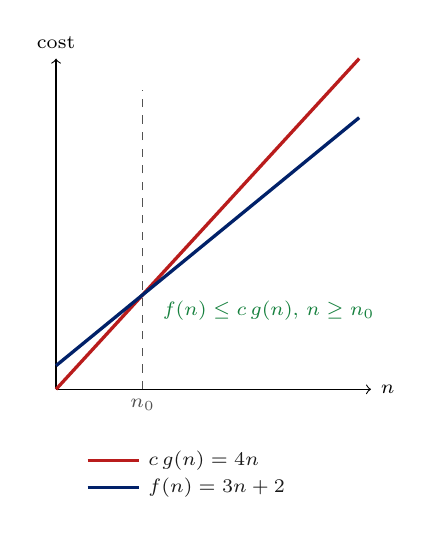
\begin{tikzpicture}[every node/.style={font=\scriptsize}]
          \draw[->] (0,0) -- (4.0,0) node[right] {$n$};
          \draw[->] (0,0) -- (0,4.2) node[above] {cost};
          \draw[very thick, color=negative] (0,0) -- (3.85,4.20);
          \draw[very thick, color=primary-blue] (0,0.30) -- (3.85,3.45);
          \draw[dashed, color=neutral] (1.10,0) -- (1.10,3.8);
          \node[color=neutral] at (1.10,-0.2) {$n_0$};
          \node[color=positive] at (2.7,1.0) {$f(n)\le c\,g(n)$, $n\ge n_0$};
          \draw[very thick, color=negative] (0.4,-0.9) -- (1.05,-0.9);
          \node[color=jet, right] at (1.05,-0.9) {$c\,g(n)=4n$};
          \draw[very thick, color=primary-blue] (0.4,-1.25) -- (1.05,-1.25);
          \node[color=jet, right] at (1.05,-1.25) {$f(n)=3n+2$};
        \end{tikzpicture}
      \end{center}
  \end{columns}
\end{frame}

\begin{frame}{Big-$O$ at Work: $T(n) = 3n + 2$}
  \begin{block}{Claim: $T(n) = 3n + 2$ is $O(n)$}
    For every $n \geq 2$, we have $3n + 2 \leq 4n$.
  \end{block}
  \begin{itemize}
    \item Choose $c = 4$ and $n_0 = 2$; then $3n + 2 \leq 4n$ holds.
    \item Therefore $T(n) = O(n)$.
    \item The exact function was $3n + 2$; the class is just $O(n)$.
  \end{itemize}
  \begin{exampleblock}{Reading it aloud}
    ``The running time is of order $n$.'' --- \muted{we have already thrown away
    the $3$ and the $2$.}
  \end{exampleblock}
\end{frame}

\begin{frame}{Big-$\Omega$: a Lower Bound}
  \begin{columns}[onlytextwidth]
    \column{0.56\textwidth}
      \begin{block}{Definition}
        $T(n) = \Omega(g(n))$ if there exist $c > 0$ and $n_0 \geq 0$ such that
        \[ T(n) \geq c \cdot g(n) \quad\text{for all } n \geq n_0. \]
      \end{block}
      \begin{itemize}
        \item ``$T(n)$ grows \emph{at least} as fast as $g(n)$, up to a constant.''
        \item $\Omega$ answers: \emph{at best, roughly how much work?}
      \end{itemize}
      \begin{exampleblock}{Example}
        $3n + 2$ is $\Omega(n)$: take $c = 3$, so $3n + 2 \geq 3n$ for all $n \geq 0$.
      \end{exampleblock}
    \column{0.44\textwidth}
      \begin{center}
        % Diagram: Big-Omega lower bound. f(n)=3n+2 is always at or above c*g(n)=3n.
        % Coordinates: x cm = n*0.55, y cm = cost*0.15.
        %   c*g(n)=3n : (0,0) -> (3.85, 3.15)  [n=7 -> 21*0.15=3.15]
        %   f(n)=3n+2 : (0,0.30) -> (3.85, 3.45) [n=7 -> 23*0.15=3.45]
        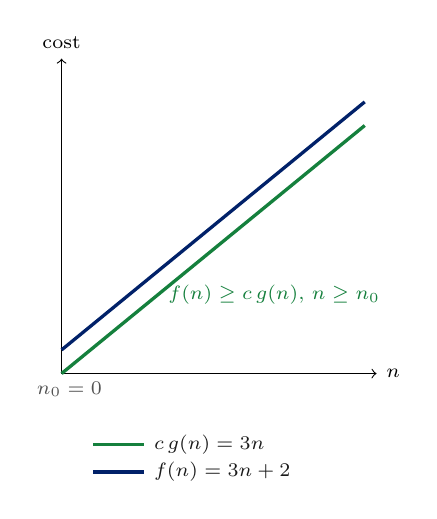
\begin{tikzpicture}[every node/.style={font=\scriptsize}]
          \draw[->] (0,0) -- (4.0,0) node[right] {$n$};
          \draw[->] (0,0) -- (0,4.0) node[above] {cost};
          \draw[very thick, color=positive] (0,0) -- (3.85,3.15);
          \draw[very thick, color=primary-blue] (0,0.30) -- (3.85,3.45);
          \node[color=neutral] at (0.1,-0.2) {$n_0=0$};
          \node[color=positive] at (2.7,1.0) {$f(n)\ge c\,g(n)$, $n\ge n_0$};
          \draw[very thick, color=positive] (0.4,-0.9) -- (1.05,-0.9);
          \node[color=jet, right] at (1.05,-0.9) {$c\,g(n)=3n$};
          \draw[very thick, color=primary-blue] (0.4,-1.25) -- (1.05,-1.25);
          \node[color=jet, right] at (1.05,-1.25) {$f(n)=3n+2$};
        \end{tikzpicture}
      \end{center}
  \end{columns}
\end{frame}

\begin{frame}{Big-$\Theta$: a Tight Bound}
  \begin{columns}[onlytextwidth]
    \column{0.56\textwidth}
      \begin{block}{Definition}
        $T(n) = \Theta(g(n))$ when $T(n)$ is \emph{both} $O(g(n))$ and $\Omega(g(n))$.
      \end{block}
      \begin{itemize}
        \item ``$T(n)$ grows \emph{exactly} like $g(n)$, up to a constant.''
        \item $\Theta$ squeezes the cost from above and below.
        \item $3n + 2$ is $\Theta(n)$: bounded below by $2n$, above by $5n$.
      \end{itemize}
      \vspace{0.1cm}
      \muted{$\Theta$ is the strongest claim of the three --- use it only when the
        two bounds actually meet.}
    \column{0.44\textwidth}
      \begin{center}
        % Diagram: Big-Theta tight bound. f(n)=3n+2 sandwiched by c1*g=2n and c2*g=5n.
        % Coordinates: x cm = n*0.55, y cm = cost*0.12 (compressed to fit legend).
        %   c2*g=5n  : (0,0) -> (3.85, 4.20)  [n=7 -> 35*0.12=4.20]
        %   f(n)=3n+2: (0,0.30) -> (3.85, 2.76) [n=7 -> 23*0.12=2.76]
        %   c1*g=2n  : (0,0) -> (3.85, 1.68)  [n=7 -> 14*0.12=1.68]
        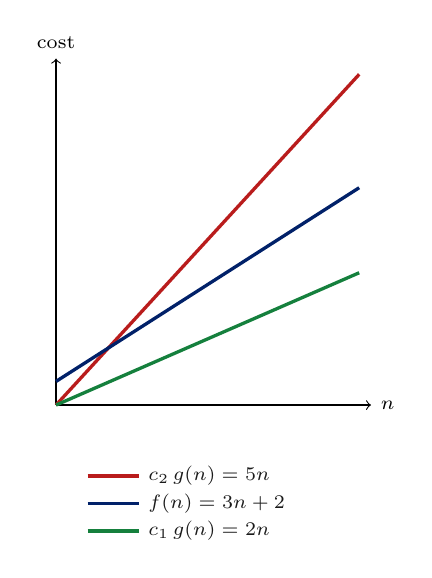
\begin{tikzpicture}[every node/.style={font=\scriptsize}]
          \draw[->] (0,0) -- (4.0,0) node[right] {$n$};
          \draw[->] (0,0) -- (0,4.4) node[above] {cost};
          \draw[very thick, color=negative] (0,0) -- (3.85,4.20);
          \draw[very thick, color=primary-blue] (0,0.30) -- (3.85,2.76);
          \draw[very thick, color=positive] (0,0) -- (3.85,1.68);
          \draw[very thick, color=negative] (0.4,-0.9) -- (1.05,-0.9);
          \node[color=jet, right] at (1.05,-0.9) {$c_2\,g(n)=5n$};
          \draw[very thick, color=primary-blue] (0.4,-1.25) -- (1.05,-1.25);
          \node[color=jet, right] at (1.05,-1.25) {$f(n)=3n+2$};
          \draw[very thick, color=positive] (0.4,-1.6) -- (1.05,-1.6);
          \node[color=jet, right] at (1.05,-1.6) {$c_1\,g(n)=2n$};
        \end{tikzpicture}
      \end{center}
  \end{columns}
\end{frame}

\begin{frame}{The Strict Siblings: $o$ and $\omega$}
  \begin{block}{When the gap is strict, not just up to a constant}
    $T(n) = o(g(n))$ means $T(n)/g(n) \to 0$; \quad
    $T(n) = \omega(g(n))$ means $T(n)/g(n) \to \infty$.
  \end{block}
  \begin{itemize}
    \item $o$ is a strict upper bound: $n = o(n^2)$, but $2n$ is \emph{not} $o(n)$.
    \item $\omega$ is a strict lower bound: $n^2 = \omega(n)$, but $2n$ is \emph{not} $\omega(n)$.
    \item The strict forms are rarely needed; we will mostly write $O$, $\Omega$, $\Theta$.
  \end{itemize}
\end{frame}

\begin{frame}{Reading Notation Correctly}
  \begin{block}{A bound must always name its case}
    ``Linear search is $O(n)$'' is incomplete --- \emph{in which case?}
  \end{block}
  \begin{itemize}
    \item \good{Linear search is $O(n)$ in the worst case.}
    \item \good{Linear search is $\Omega(1)$ in the best case.}
    \item \bad{Binary search is $O(\log n)$} --- \muted{no case stated.}
    \item \bad{$T(n) = O(n)$, so exactly $n$ steps} --- \muted{confuses a class with a count.}
  \end{itemize}
  \key{Pair every complexity claim with the case, and name the operation.}
\end{frame}

\transitionslide{Now apply the vocabulary to our two searches.}

% =============================================================================
% ACT 3 --- TWO SEARCHES, TWO COSTS
% =============================================================================
\section{Two Searches, Two Costs}

\sectiondivider{Section 3}{Two Searches, Two Costs}

\begin{frame}{Linear Search, Analysed}
  \begin{block}{Cost of \texttt{linear\_search}}
    Basic operation: the comparison \texttt{A[i] == key}.
  \end{block}
  \begin{itemize}
    \item \key{Worst case}: $n$ comparisons --- the trace: \texttt{key} absent,
      every \texttt{A[i]} examined once.
    \item \key{Best case}: $1$ comparison --- \texttt{key == A[0]}.
    \item \key{Average case}: $\frac{n+1}{2} = \Theta(n)$ comparisons.
  \end{itemize}
  \vspace{0.15cm}
  \muted{Every claim above names its case, and each is matched to the input
    that exhibits it.}
\end{frame}

\begin{frame}{Binary Search Needs a Sorted Table}
  \begin{block}{Precondition (an invariant, not an option)}
    Binary search is only correct when the array is sorted. On an unsorted
    array it can silently return a wrong answer.
  \end{block}
  \begin{itemize}
    \item The sorted order is \emph{what makes halving valid}: after one
      comparison we can discard an entire half.
    \item Keeping the table sorted is itself a cost --- the price we pay for
      fast lookups later.
    \item \muted{This is the anti-pattern to guard: never apply binary search
      without first stating the sorted precondition.}
  \end{itemize}
\end{frame}

\begin{frame}[fragile]{Binary Search}
  \begin{block}{Jump to the middle, then discard a half}
\begin{semiverbatim}
int binary_search(int A[], int n, int key) \{
    int lo = 0, hi = n - 1;
    while (lo <= hi) \{
        int mid = lo + (hi - lo) / 2;
        if (A[mid] == key) return mid;
        else if (A[mid] < key) lo = mid + 1;
        else                  hi = mid - 1;
    \}
    return -1;
\}
\end{semiverbatim}
  \end{block}
  \begin{itemize}
    \item Each pass compares \texttt{A[mid]} and shrinks \texttt{[lo, hi]} by half.
    \item \texttt{A} must already be sorted, in ascending order.
  \end{itemize}
\end{frame}

\begin{frame}{Binary Search: the Halving Picture}
  \begin{center}
    % Diagram: sorted array A[0..8]; lo/mid/hi pointers; search for key = 68.
    % Coordinates: (x, y)
    %   cell i at x = 0.9*i (i = 0..8), y = 0, w = 0.85cm, h = 0.75cm
    %   pointer labels lo/mid/hi at y = 1.15, arrows down to cell tops
    %   index labels at y = -0.62 (below the cells, clear of them)
    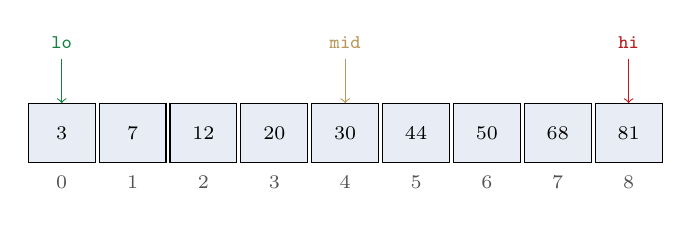
\begin{tikzpicture}[every node/.style={font=\scriptsize}]
      \foreach \i/\v in {0/3,1/7,2/12,3/20,4/30,5/44,6/50,7/68,8/81} {
        \node[draw, minimum width=0.85cm, minimum height=0.75cm, fill=light-bg]
          (\i) at (0.9*\i, 0) {\v};
      }
      \foreach \i in {0,...,8} {
        \node[text=neutral] at (0.9*\i, -0.62) {\i};
      }
      \node[text=positive] (lo) at (0, 1.15) {\texttt{lo}};
      \node[text=primary-gold] (mid) at (0.9*4, 1.15) {\texttt{mid}};
      \node[text=negative] (hi) at (0.9*8, 1.15) {\texttt{hi}};
      \draw[->, color=positive] (lo.south) -- (0.north);
      \draw[->, color=primary-gold] (mid.south) -- (4.north);
      \draw[->, color=negative] (hi.south) -- (8.north);
    \end{tikzpicture}
  \end{center}
  \begin{itemize}
    \item \texttt{mid = lo + (hi - lo) / 2} lands on index $4$ (value $30$).
    \item $30 < 68$, so the left half is discarded and \texttt{lo} jumps to $5$.
  \end{itemize}
\end{frame}

\begin{frame}{Binary Search Trace (key = 68)}
  \begin{center}
  \begin{tabular}{ccccc}
    \toprule
    \textbf{pass} & \texttt{lo} & \texttt{hi} & \texttt{mid} & \texttt{A[mid]} \\
    \midrule
    1 & 0 & 8 & 4 & $30 < 68$ \\
    2 & 5 & 8 & 6 & $50 < 68$ \\
    3 & 7 & 8 & 7 & $68 = 68$ --- found \\
    \bottomrule
  \end{tabular}
  \end{center}
  \begin{itemize}
    \item Three passes to find \texttt{key = 68} among $n = 9$ values.
    \item A linear scan would check $7$ of the $9$ cells (worst case: all $9$).
  \end{itemize}
  \muted{Each pass discards half the remaining interval --- that is the engine
    of the logarithmic bound.}
\end{frame}

\begin{frame}{Binary Search, Analysed}
  \begin{block}{Cost of \texttt{binary\_search}}
    Basic operation: the comparison \texttt{A[mid] == key}.
  \end{block}
  \begin{itemize}
    \item Each pass halves the interval $[\,\texttt{lo}, \texttt{hi}\,]$; after
      $k$ passes at most $\lceil n/2^k \rceil$ elements remain.
    \item The loop stops when the interval is empty, so the number of passes is
      about $\log_2 n$.
  \end{itemize}
  \vspace{0.15cm}
  \key{Binary search is $O(\log n)$ in the worst case --- and $\Omega(1)$ in the
    best case (key at \texttt{A[mid]} on the first pass).}
  \muted{$\log$ is the base-2 logarithm here; its base is a constant factor,
    which asymptotic notation drops anyway.}
\end{frame}

\begin{frame}[fragile]{A Nested Loop: Checking for Duplicates}
  \begin{block}{Does the symbol table hold the same name twice?}
\begin{semiverbatim}
for (int i = 0; i < n; i++)
    for (int j = i + 1; j < n; j++)
        if (A[i] == A[j])
            return 1;  /* duplicate found */
\end{semiverbatim}
  \end{block}
  \begin{itemize}
    \item The inner loop runs $n - i - 1$ times for each $i$.
    \item Total comparisons: $\sum_{i=0}^{n-2}(n-i-1) = \frac{n(n-1)}{2}$.
    \item This is $\Theta(n^2)$ --- \emph{in every case}, since the loop always
      runs to completion unless a duplicate is found.
  \end{itemize}
\end{frame}

\begin{frame}{The Numbers Side by Side}
  \begin{center}
  \begin{tabular}{rrrrr}
    \toprule
    $n$ & $\log_2 n$ & $n$ & $n \log_2 n$ & $n^2$ \\
    \midrule
    $10$      & $\approx 3$   & $10$        & $\approx 33$    & $10^2$ \\
    $10^3$    & $\approx 10$  & $10^3$      & $\approx 10^4$  & $10^6$ \\
    $10^6$    & $\approx 20$  & $10^6$      & $\approx 2\cdot10^7$ & $10^{12}$ \\
    \bottomrule
  \end{tabular}
  \end{center}
  \begin{block}{What the table says}
    As $n$ grows, $\log n$ barely moves while $n^2$ explodes --- the difference
    between a search that is practical and one that is not.
  \end{block}
\end{frame}

\begin{frame}{The Symbol Table Payoff}
  \begin{block}{The same table, three later homes}
    Our calculator's identifier lookup, analysed as $n$ grows:
  \end{block}
  \begin{itemize}
    \item \key{Unsorted list} (Week 6): lookup is $O(n)$ worst case --- scan it all.
    \item \key{Sorted array}: lookup is $O(\log n)$ worst case --- but keeping it
      sorted costs on every insert.
    \item \key{Hash table} (Week 10): lookup is $O(1)$ expected --- the whole
      reason we will want one.
  \end{itemize}
  \vspace{0.15cm}
  \muted{Week 2 gives us the vocabulary to make this trade-off precise; Weeks
    6 and 10 will act on it.}
\end{frame}

\transitionslide{Time is only half the bill --- memory matters too.}

% =============================================================================
% ACT 4 --- SPACE
% =============================================================================
\section{Space}

\sectiondivider{Section 4}{Space}

\begin{frame}{Space Complexity $S(n)$}
  \begin{block}{Definition}
    $S(n)$ is the amount of memory an algorithm uses beyond its input --- its
    \emph{auxiliary} space --- as a function of $n$.
  \end{block}
  \begin{itemize}
    \item \key{Input space}: the $n$ elements themselves --- counted separately.
    \item \key{Auxiliary space}: the extra working memory the algorithm needs.
    \item $S(n)$ is stated the same way as $T(n)$, in asymptotic classes.
  \end{itemize}
  \vspace{0.15cm}
  \muted{We separate the two because ``uses $n$ cells'' is uninteresting when
    the input already has $n$ cells; the extra is the real question.}
\end{frame}

\begin{frame}{Space of Our Examples}
  \begin{block}{Auxiliary space, one constant at a time}
    Each of today's algorithms keeps only a handful of local variables.
  \end{block}
  \begin{itemize}
    \item \texttt{linear\_search}: one index \texttt{i} --- auxiliary space $O(1)$.
    \item \texttt{binary\_search}: three indices \texttt{lo}, \texttt{hi},
      \texttt{mid} --- auxiliary space $O(1)$.
    \item A \emph{recursive} binary search would instead use $O(\log n)$ stack
      frames --- the recursion depth.
  \end{itemize}
  \begin{exampleblock}{Why it matters}
    $O(1)$ auxiliary space means the extra memory does not grow with $n$ --- a
    property we will price carefully when Week 9 compares in-place and
    merge-sort. \muted{The pointer intuition is Week 1's: each variable is one
    cell, wherever it lives.}
  \end{exampleblock}
\end{frame}

% =============================================================================
% ACT 5 --- WRAP UP
% =============================================================================
\section{Summary}

\begin{frame}{Three Common Mistakes}
  \begin{itemize}
    \item \bad{Treating $T(n) = O(n)$ as an exact count} --- $O(n)$ is a class,
      not ``$n$ steps.''
    \item \bad{Stating a bound with no case} --- ``$O(n)$'' without worst/best/
      average leaves the claim unfalsifiable.
    \item \bad{Mixing up $O$ and $\Theta$} --- $O$ is an upper bound; only $\Theta$
      says the growth matches exactly.
  \end{itemize}
  \begin{exampleblock}{The habit}
    Name the operation, give the bound, state the case, and point to the input
    that exhibits it.
  \end{exampleblock}
\end{frame}

\begin{frame}{Week 2 Summary}
  \begin{itemize}
    \item \key{Cost model}: count a basic operation as a function of $n$.
    \item \key{$T(n)$}: the exact cost function; \key{$S(n)$}: the auxiliary space.
    \item \key{Asymptotic classes}: $O$ (upper), $\Omega$ (lower), $\Theta$ (tight),
      with $o$ and $\omega$ as the strict forms.
    \item \key{Cases}: best, worst, average --- orthogonal to the bound, always
      stated with it.
    \item \key{Our two searches}: linear $O(n)$ worst case vs.\ binary $O(\log n)$
      worst case; a nested loop is $\Theta(n^2)$.
  \end{itemize}
  \vspace{0.15cm}
  \begin{exampleblock}{Next week}
    Arrays and the Stack ADT --- the first structure we will analyse end to end.
  \end{exampleblock}
\end{frame}

\begin{frame}{Before You Go: Predict}
  \begin{block}{Doubling the table}
    The calculator's symbol table doubles from $n$ to $2n$ names. Which lookup
    grows how?
  \end{block}
  \begin{enumerate}
    \item A linear scan: roughly how much slower?
    \item A binary search: roughly how much slower?
    \item A duplicate check with the nested loop: roughly how much slower?
  \end{enumerate}
  \muted{Your answers --- ``doubles'', ``one extra pass'', ``four times'' --- are
    the whole point of the asymptotic vocabulary.}
\end{frame}

\begin{frame}[allowframebreaks]{References}
  \footnotesize
  \bibliographystyle{plain}
  \bibliography{../../Bibliography_base}
\end{frame}

\end{document}
